\documentclass{beamer}

\beamertemplatenavigationsymbolsempty
\setbeamerfont{page number in head/foot}{size=\small}
\setbeamertemplate{footline}[frame number]
\usefonttheme[onlymath]{serif}

\usepackage[utf8]{inputenc}

\usepackage[T1]{fontenc}
\usepackage[english]{babel}
%\usepackage[utf8]{inputenc}

\usepackage{tikz}
\usetikzlibrary{calc}
\usetikzlibrary{arrows, backgrounds}
\usetikzlibrary{matrix, arrows.meta}
\usetikzlibrary{decorations.pathreplacing}
\usetikzlibrary{positioning, fit, shapes}

\usepackage{ifthen}

%\usetikzlibrary{external}
%\tikzexternalize[prefix=tikz/]

\newcommand{\backupbegin}{
   \newcounter{finalframe}
   \setcounter{finalframe}{\value{framenumber}}
}
\newcommand{\backupend}{
   \setcounter{framenumber}{\value{finalframe}}
}

% Scale all pgf plots, not only coordinates
\usepackage{adjustbox}

%\usepackage{amsfonts}
%\usepackage{amsmath}
%\usepackage{amsthm}
\usepackage{bm}

\usepackage{pgfplots}
\pgfplotsset{compat=1.16}
\usepgfplotslibrary{groupplots}

% Used for split environment
\usepackage{amsmath}
% Separate rows in align environment by this amount
\addtolength{\jot}{1em}

\usepackage{graphicx}
\graphicspath{{../fig/} {fig/}}
\usepackage{subfig}
\usepackage{wrapfig}

% Clickable links
\usepackage{hyperref}
\hypersetup{
	colorlinks,
	citecolor=black,
	filecolor=black,
	linkcolor=black,
	urlcolor=black
}

\usepackage[pdf]{graphviz}

%\usepackage[dvipsnames]{xcolor}
\usepackage{listings}

\lstset{
	language=c,
  basicstyle=\small\ttfamily,  % the size of the fonts that are used for the code
	numbers=none,                   % where to put the line-numbers
  inputencoding=latin1,
  numberstyle=\tiny,  % the style that is used for the line-numbers
  stepnumber=1,                   % the step between two line-numbers. If it's
				    %1, each line 
                                  % will be numbered
  %numbersep=5pt,                  % how far the line-numbers are from the code
  backgroundcolor=\color{white},      % choose the background color.
  showspaces=false,               % show spaces adding particular underscores
  showstringspaces=false,         % underline spaces within strings
  showtabs=false,      % show tabs within strings adding particular underscores
	frame=none,                   % adds a frame around the code
  rulecolor=\color{black},        % if not set, the frame-color may be changed
				   % on line-breaks within not-black text (e.g.
				   % comments (green here))
	tabsize=6,                      % sets default tabsize to 2 spaces
  columns=fullflexible,
  extendedchars=true,
  captionpos=b,                   % sets the caption-position to bottom
  breaklines=true,                % sets automatic line breaking
  breakatwhitespace=false,        % sets if automatic breaks should only happen
				    %at whitespace
  title=\lstname,                   % show the filename of files included with
				    %\lstinputlisting;
                                  % also try caption instead of title
  keywordstyle=\color{blue},          % keyword style
	commentstyle=\color{gray},       % comment style
	stringstyle=\color{brown},         % string literal style
	escapeinside={|*}{*|},            % if you want to add LaTeX within your code
	morecomment=[l][\color{purple}]{\#},
	moredelim=[il][\color{purple}]{@},
	abovecaptionskip=-15pt
%	belowcaptionskip=-15pt
}


\usepackage{csquotes}

\usepackage{siunitx}

\usepackage{multicol}

\usepackage{epigraph}
\setlength{\epigraphwidth}{0.7\textwidth}

\usepackage{caption}
\captionsetup{font=footnotesize}

% Macros para ayudar a la redacción
% Vector
\newcommand*\mat[1]{ \begin{pmatrix} #1 \end{pmatrix}}
\newcommand*\arr[1]{ \begin{bmatrix} #1 \end{bmatrix}}
\newcommand*\V[1]{\bm{#1}}
\newcommand{\E}{\V{E}}
\newcommand{\rhog}{\rho_\text{ghost}}
\newcommand{\F}{\V{F}}
\newcommand{\B}{\V{B}}
\renewcommand*{\v}{\V{v}}
\newcommand{\x}{\V{x}}
\newcommand{\dt}{\Delta t}
\newcommand{\dx}{\Delta x}
\newcommand*\neigh[1]{\mathcal{N}(#1)}

% Norm
\newcommand\norm[1]{\left\lVert#1\right\rVert}

\title{How TAP works\\{\small Example with the FFT in cpic.}}
\author{Rodrigo Arias Mallo}
\institute{Barcelona Supercomputing Center (BSC)}
\date{\today}





\tikzset{
	red-frame/.style={white}
}

% Running style for the nodes
\tikzset{
	running/.style={fill=green!30}
}

\tikzset{
	stopped/.style={fill=red!30}
}

% The threads are defined in a matrix called t, where each thread is labeled
% from t0 to t3, so we can reference them later.

\tikzset{
%	master/.pic = {
	pics/master/.style args={#1/#2}{
		code={
			\matrix[
				ampersand replacement=\&,
				nodes={#2,draw,circle,inner sep=0mm,minimum size=8mm},
				column sep=3mm,
	%				left=1cm of O,
			] (n#1-t)
			{
				\node (n#1-t0) {$t_0$}; \&
				\node (n#1-t1) {$t_1$}; \&
				\node (n#1-t2) {$t_2$}; \&
				\node (n#1-t3) {$t_3$}; \\
			};

			%\node[draw,fit=(t0) (t3),inner sep=1mm,rounded corners=4mm] (master) {};
			%\node[draw,fit=(t0) (t3),inner sep=0.5mm,ellipse] (master) {};
			\node[
				thick,
				draw=blue,
				fit=(n#1-t0) (n#1-t3),circle
			] (n#1-master) {};

			\node[below=0.5em of n#1-master.north]
				{Rank \pgfmathparse{int(#1-1)}\pgfmathresult};
		}
	}
}

% Same for the workers, we have w for all of them, and w0 to w3 for each one.
\tikzset{
%	workers/.pic = {
	pics/workers/.style args={#1/#2}{
		code={
			\matrix[
				ampersand replacement=\&,
				nodes={
					#2,
					%double,
					%double circle={1mm}{red}
					%double distance=1mm,
					%draw=red,
					draw,
					anchor=center,
					circle,
					inner sep=0mm,
					minimum size=8mm
				},
				column sep=6mm] (n#1-w) {
				\node (n#1-wt0) {$w_0$}; \&
				\node (n#1-wt1) {$w_1$}; \&
				\node (n#1-wt2) {$w_2$}; \&
				\node (n#1-wt3) {$w_3$}; \\
			};

			\foreach \i in {0,...,3}
			{
				\node[
					thick,
					circle,
					draw=red,
					minimum size=11mm,
					anchor=center
				] (n#1-w\i) at (n#1-wt\i) {}; \&
				\node[below=1mm of n#1-w\i]
					{\footnotesize Rank \pgfmathparse{int((#1-1)*4+\i)}\pgfmathresult};
			}

			%\node[right=1mm of w] {Workers};
		}
	}
}

% Same for CPUs, with c for all and c0 to c3 for each one.
\tikzset{
	pics/cpus/.style args={#1}{
		code={
		% Draw the CPUs
			\matrix[
				ampersand replacement=\&,
				matrix of nodes,
				nodes={
					draw,
					thick,
					rectangle,
					inner sep=0mm,
					minimum size=9mm
				},
				outer sep=0mm,
				inner sep=0mm,
				column sep=1mm
			] (n#1-c)
			{
				\node (n#1-c0) {$c_0$}; \&
				\node (n#1-c1) {$c_1$}; \&
				\node (n#1-c2) {$c_2$}; \&
				\node (n#1-c3) {$c_3$}; \\
			};
		}
	}
}

\tikzset{
	global/.style = {white}
}
\tikzset{
	shared/.style = {black}
}

\tikzset{
	pics/mem/.style args={#1/#2}{
		code={

			\matrix[
				row 1/.style={nodes={draw=white}},
				row 6/.style={nodes={draw=white}},
				nodes={
					anchor=center,
					dashed,
					draw=gray,
					%draw,
					#2,
					rectangle,
					minimum width=4cm,
					minimum height=2em,
					outer sep=0mm,
					inner sep=0mm,
				},
				outer sep=0mm,
				inner sep=0mm,
				row sep =-\pgflinewidth,
				column sep = -\pgflinewidth,
				column sep=0mm,
			] (n#1-m)
			{
				\node (n#1-mp) {$\cdots$}; \\
				\node (n#1-m0) {$m_0$}; \\
				\node (n#1-m1) {$m_1$}; \\
				\node (n#1-m2) {$m_2$}; \\
				\node (n#1-m3) {$m_3$}; \\
				\node (n#1-mn) {$\cdots$}; \\
			};

			\ifthenelse{\equal{#2}{global}}{
				\node[below=-3mm of n#1-m.center] {Memory};
			}
			{
				\node[draw,
					thick,
					inner sep=0mm,
					fit=(n#1-m0)(n#1-m3),
				] (n#1-sm)	{};
			}
		}
	}
}

% Same for CPUs, with c for all and c0 to c3 for each one.
\tikzset{
	%node/.pic = {
	pics/node/.style args={#1/#2}{
		code={

			\coordinate (n#1-O) at (0,0);


			% Draw the CPUs
			\pic[above=18mm of n#1-O] {cpus={#1}};

			% Draw the memory
			\pic [below=2mm of n#1-c] {mem={#1/#2}};

			%\draw (m.north west) rectangle (m.south east);
			\node[inner sep=0mm, draw=gray,fit=(n#1-m)] {};
			\node[above=2mm of n#1-c] (n#1-text) {Node #1};

			\node (n#1) [
				inner sep=2mm,
				rounded corners=2mm,
				draw=gray,
				fit=(n#1-c)(n#1-m)(n#1-text)
			] {};
		}
	}
}

\tikzset{
	canvas/.pic = {
		% Draw the canvas
		\draw[red-frame] (-10,-8) rectangle (10,8);
	}
}

\tikzset{
	pics/cluster/.style args={#1}{
		code={
			\coordinate (O) at (0,0);
			\pic[above=40mm of O] {node={1/#1}};
			\pic[below=40mm of O] {node={2/#1}};
		}
	}
}

\tikzset{
	pics/base/.style args={#1}{
		code={
			% The center will be the origin
			\coordinate (O) at (0,0);
			\pic {canvas};

			% Draw the clusters
			\pic[right=6cm of O] {cluster={#1}};

			\draw[dotted] (-10,0) -- (10,0);

			\draw[<->] (n1) -- (n2) node [midway,right] {Network};
		}
	}
}

\tikzset{
	pics/full/.style args={#1/#2}{
		code={
			\pic {base};
			% Master process with 4 threads
			\pic[left=7cm of n1] {master={1/#1}};
			\pic[left=7cm of n2] {master={2/#1}};
			%\draw[thick,blue] (n1-master) -- (n2-master);

			% Draw the workers
			\pic[below left=1cm and 1cm of n1-m.west] {workers={1/#2}};
			\pic[below left=1cm and 1cm of n2-m.west] {workers={2/#2}};
		}
	}
}


\begin{document}

\frame{\titlepage}

\begin{frame}{TAP}


\begin{figure}
\centering
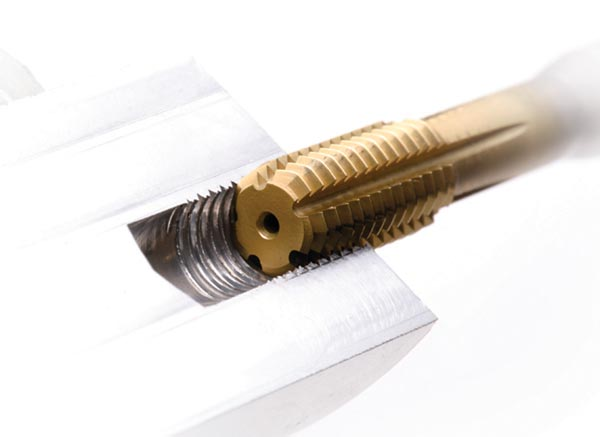
\includegraphics[width=0.5\textwidth]{tap-tool.jpg}
\end{figure}

The name TAP comes from the tap tool used to cut threads into parts. The idea is 
to take a application and force it to support ``threading'' by creating one 
process for each CPU.

\end{frame}

\begin{frame}{Use case: Plasma simulation}

The technique comes from a problem observed in the spectral solver used in 
plasma simulation, where the FFTW library is used. The performance when using 
the threads implementation is very bad.

\vspace{1em}

The solver becomes the bottleneck of the simulation. However by creating more 
processes, the FFTW can improve the performance, but the rest of the simulation 
doesn't benefit.

\end{frame}

\begin{frame}{Problem observed}

\begin{figure}
\centering
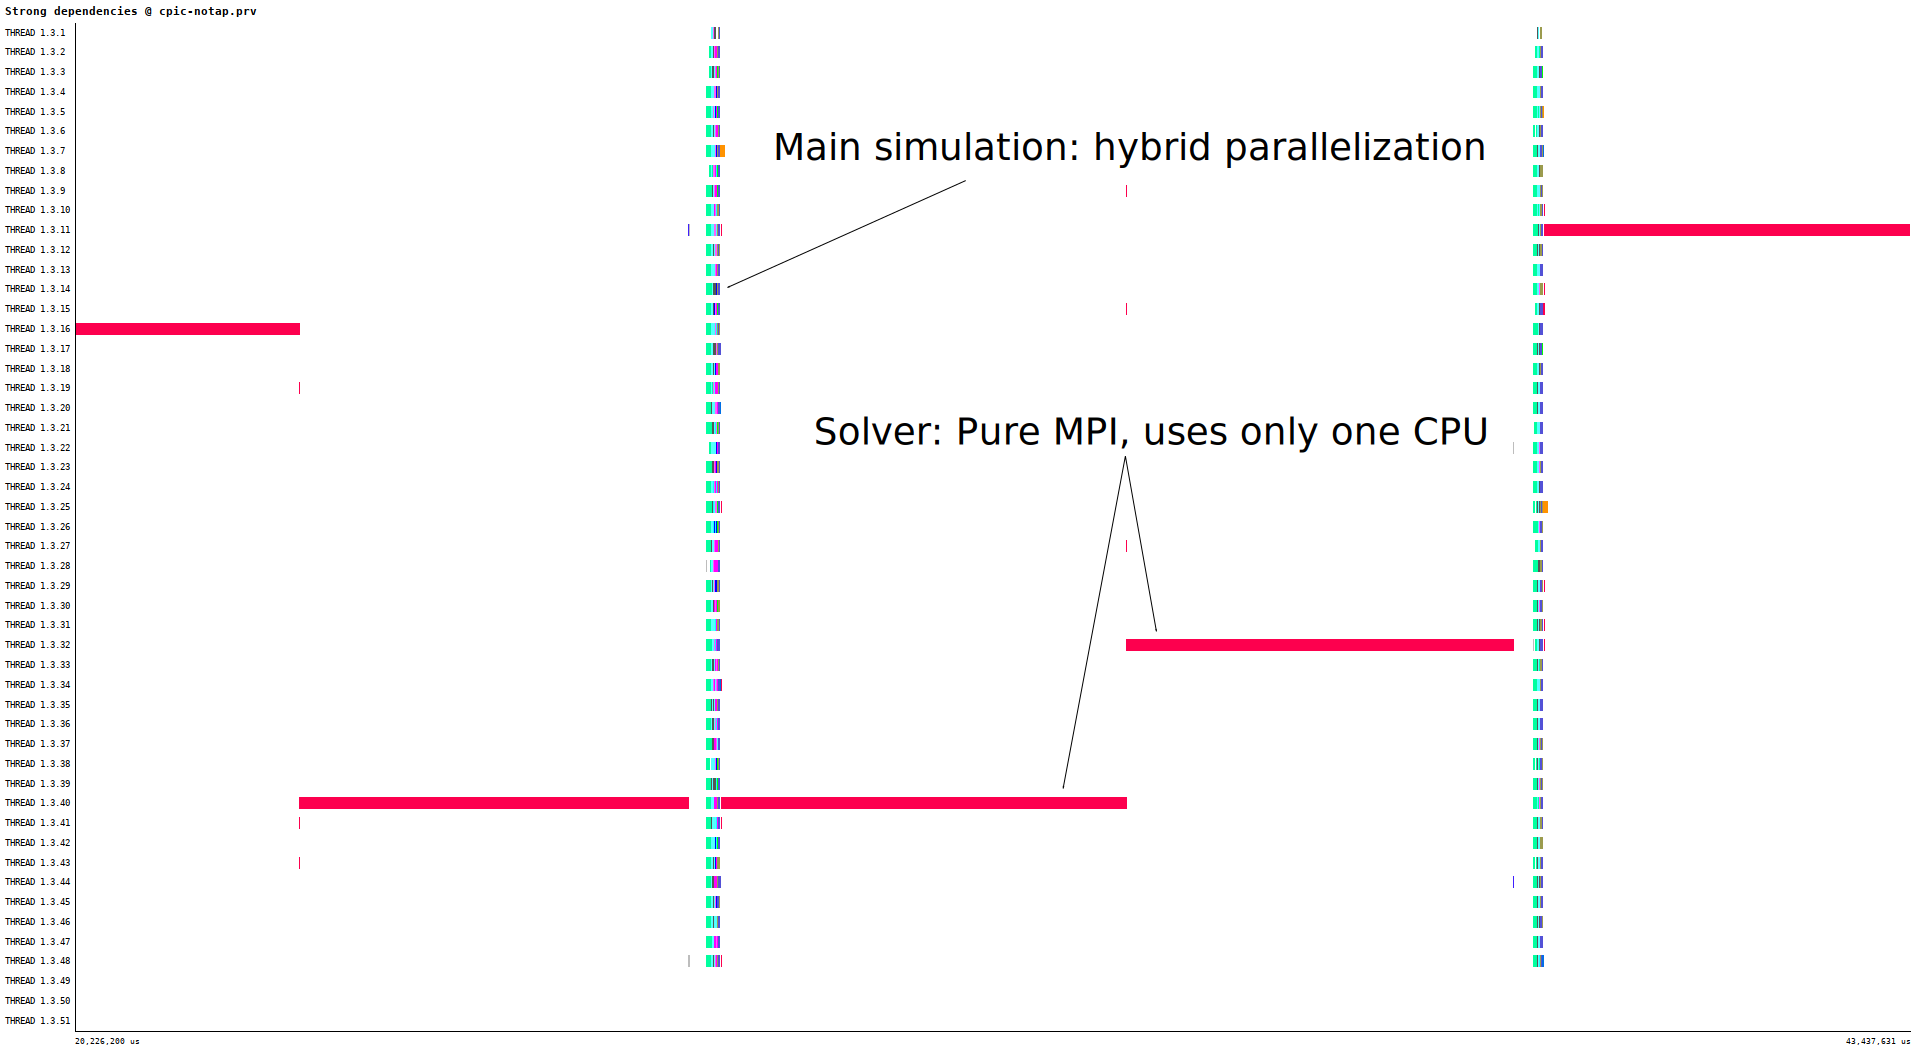
\includegraphics[width=\textwidth]{tap/notap}
\caption{A trace of the simulation with two iterations is shown, focused only in 
one node with 48 CPUs.}
\end{figure}


\end{frame}

\begin{frame}{Proposed solution: TAP}

The idea is to create more processes only for the solver, while the main 
simulation continues with one process per node.

\vspace{1em}

An in depth example with 2 nodes is shown, where the hybrid part of the 
simulation runs in the master process, and the solver in the workers.

\end{frame}

\begin{frame}[fragile]
\begin{figure}[h]
\begin{adjustbox}{max totalsize={\textwidth}{\textheight},center}
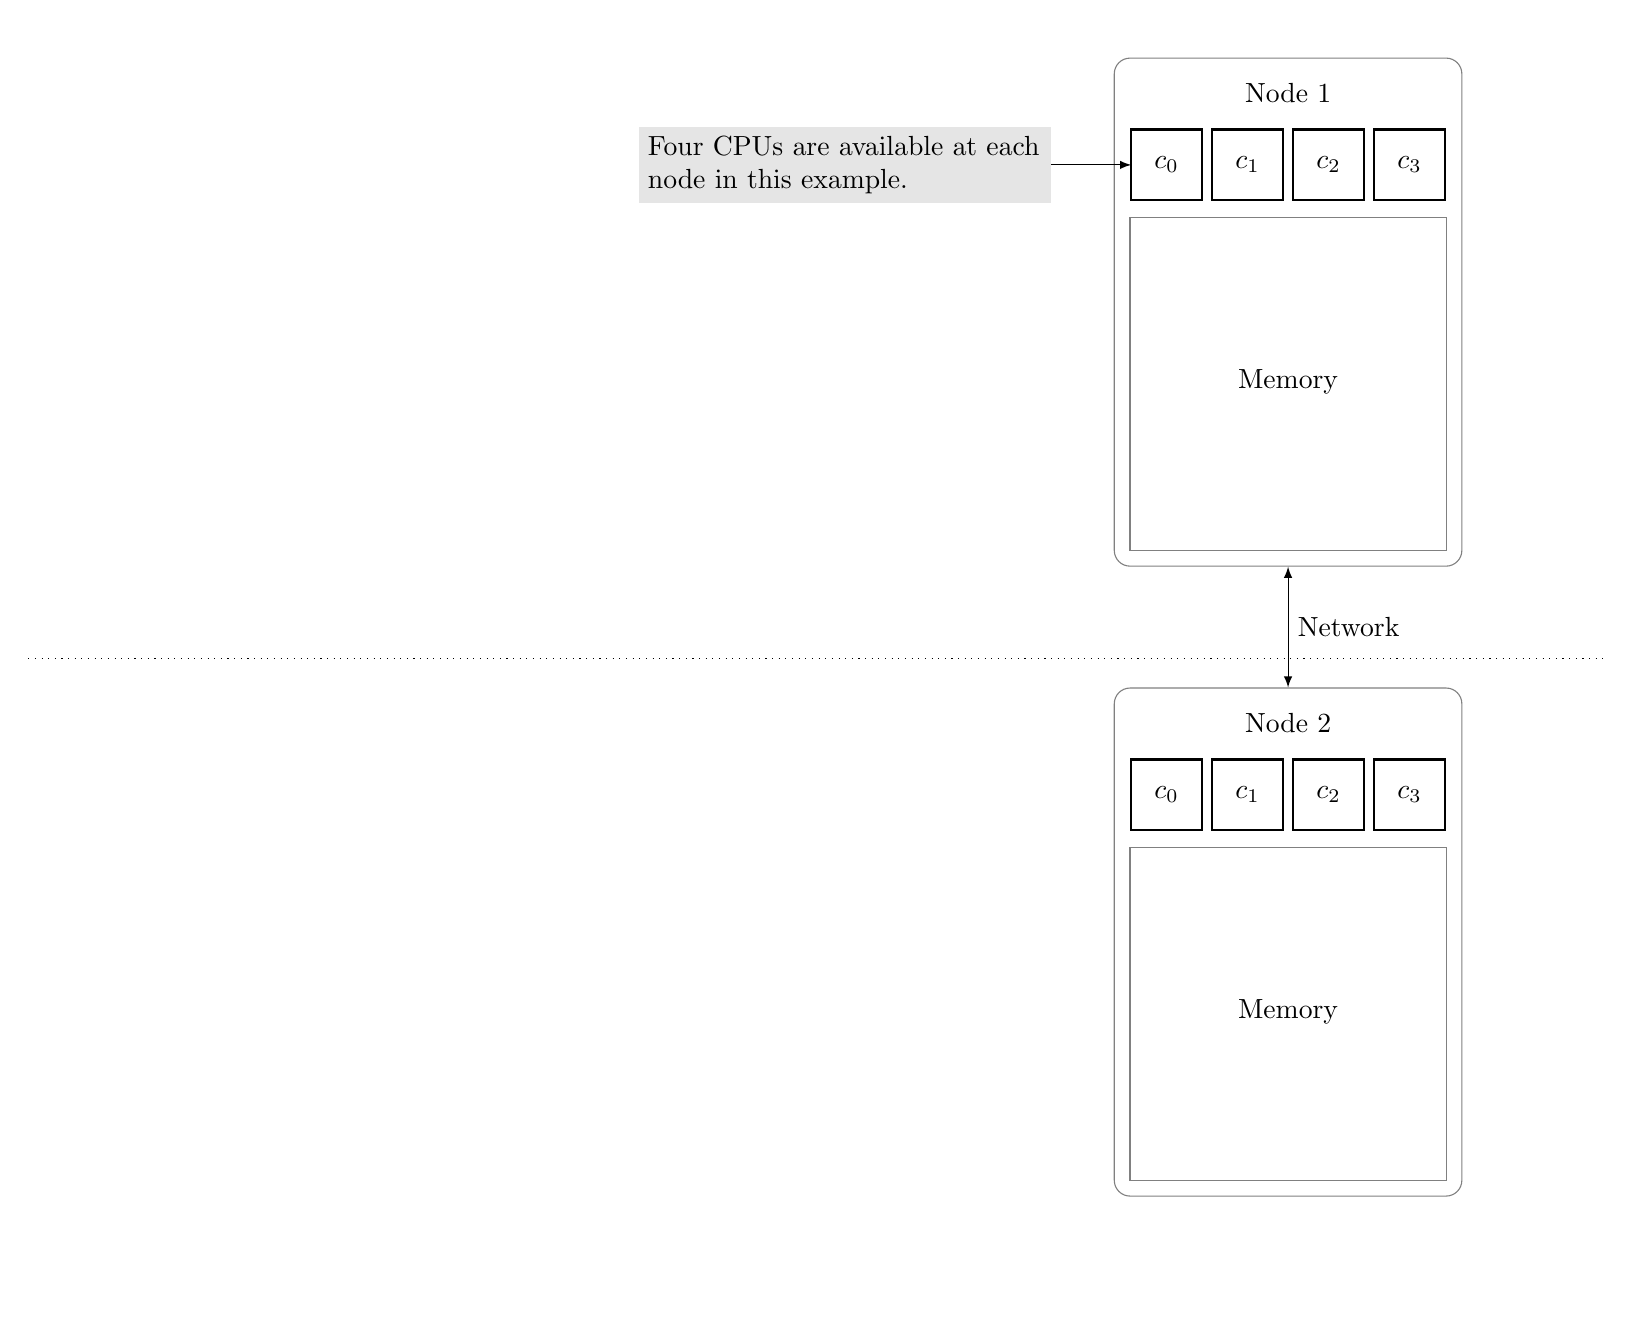
\begin{tikzpicture}[>=latex]
	\pic {base={global}};

	\node (text) [fill=gray!20,left=1cm of n1-c,text width=5cm]
		{Four CPUs are available at each node in this example.};

	\draw[->] (text) -- (n1-c0);

\end{tikzpicture}
\end{adjustbox}
\end{figure}
\end{frame}

\begin{frame}[fragile]
\begin{figure}[h]
\begin{adjustbox}{max totalsize={\textwidth}{\textheight},center}
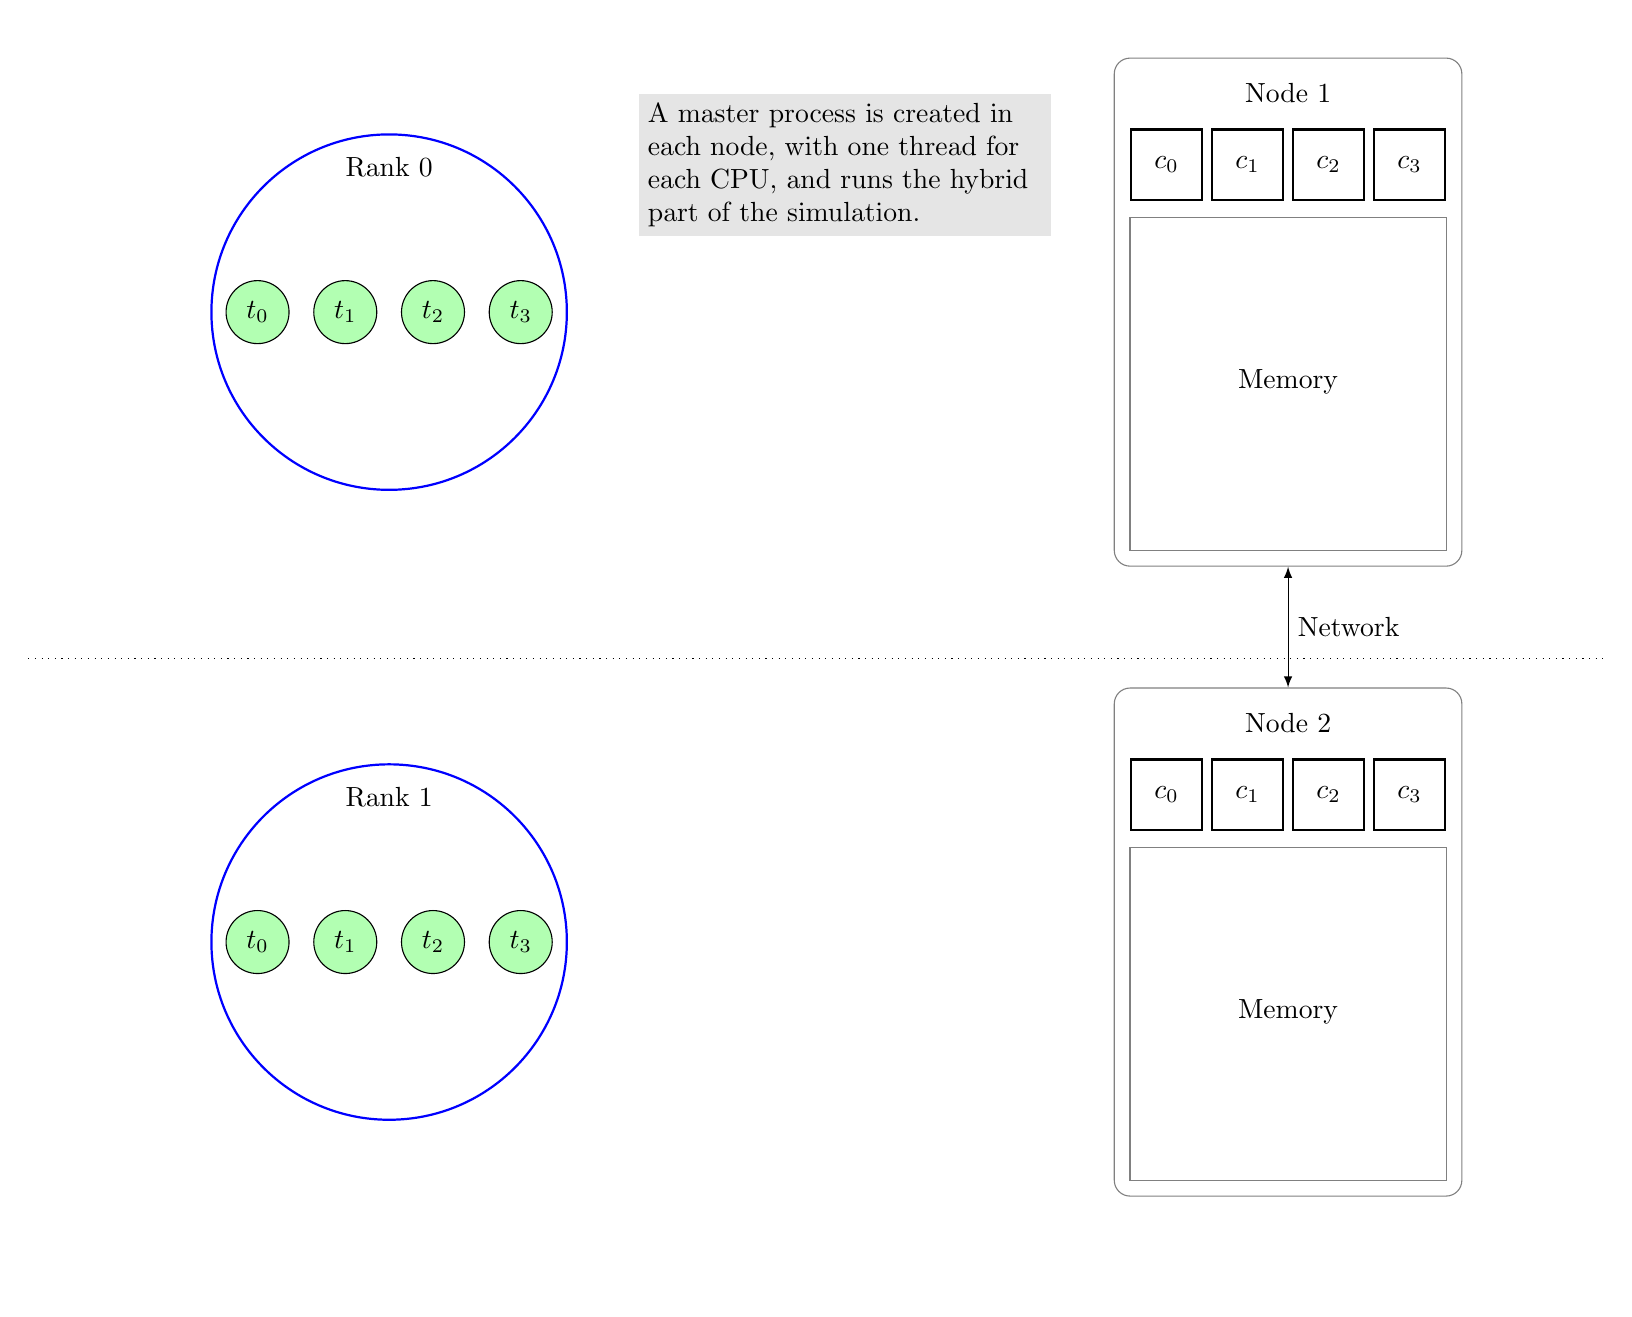
\begin{tikzpicture}[
		>=latex,
	]

	\pic {base={global}};

	% Master process with 4 threads
	\pic[left=7cm of n1] {master={1/running}};
	\pic[left=7cm of n2] {master={2/running}};

	\node (text) [fill=gray!20,left=1cm of n1-c,text width=5cm]
		{A master process is created in each node, with one thread for each CPU, and 
		runs the hybrid part of the simulation.};

\end{tikzpicture}
\end{adjustbox}
\end{figure}
\end{frame}

\begin{frame}[fragile]
\begin{figure}[h]
\begin{adjustbox}{max totalsize={\textwidth}{\textheight},center}
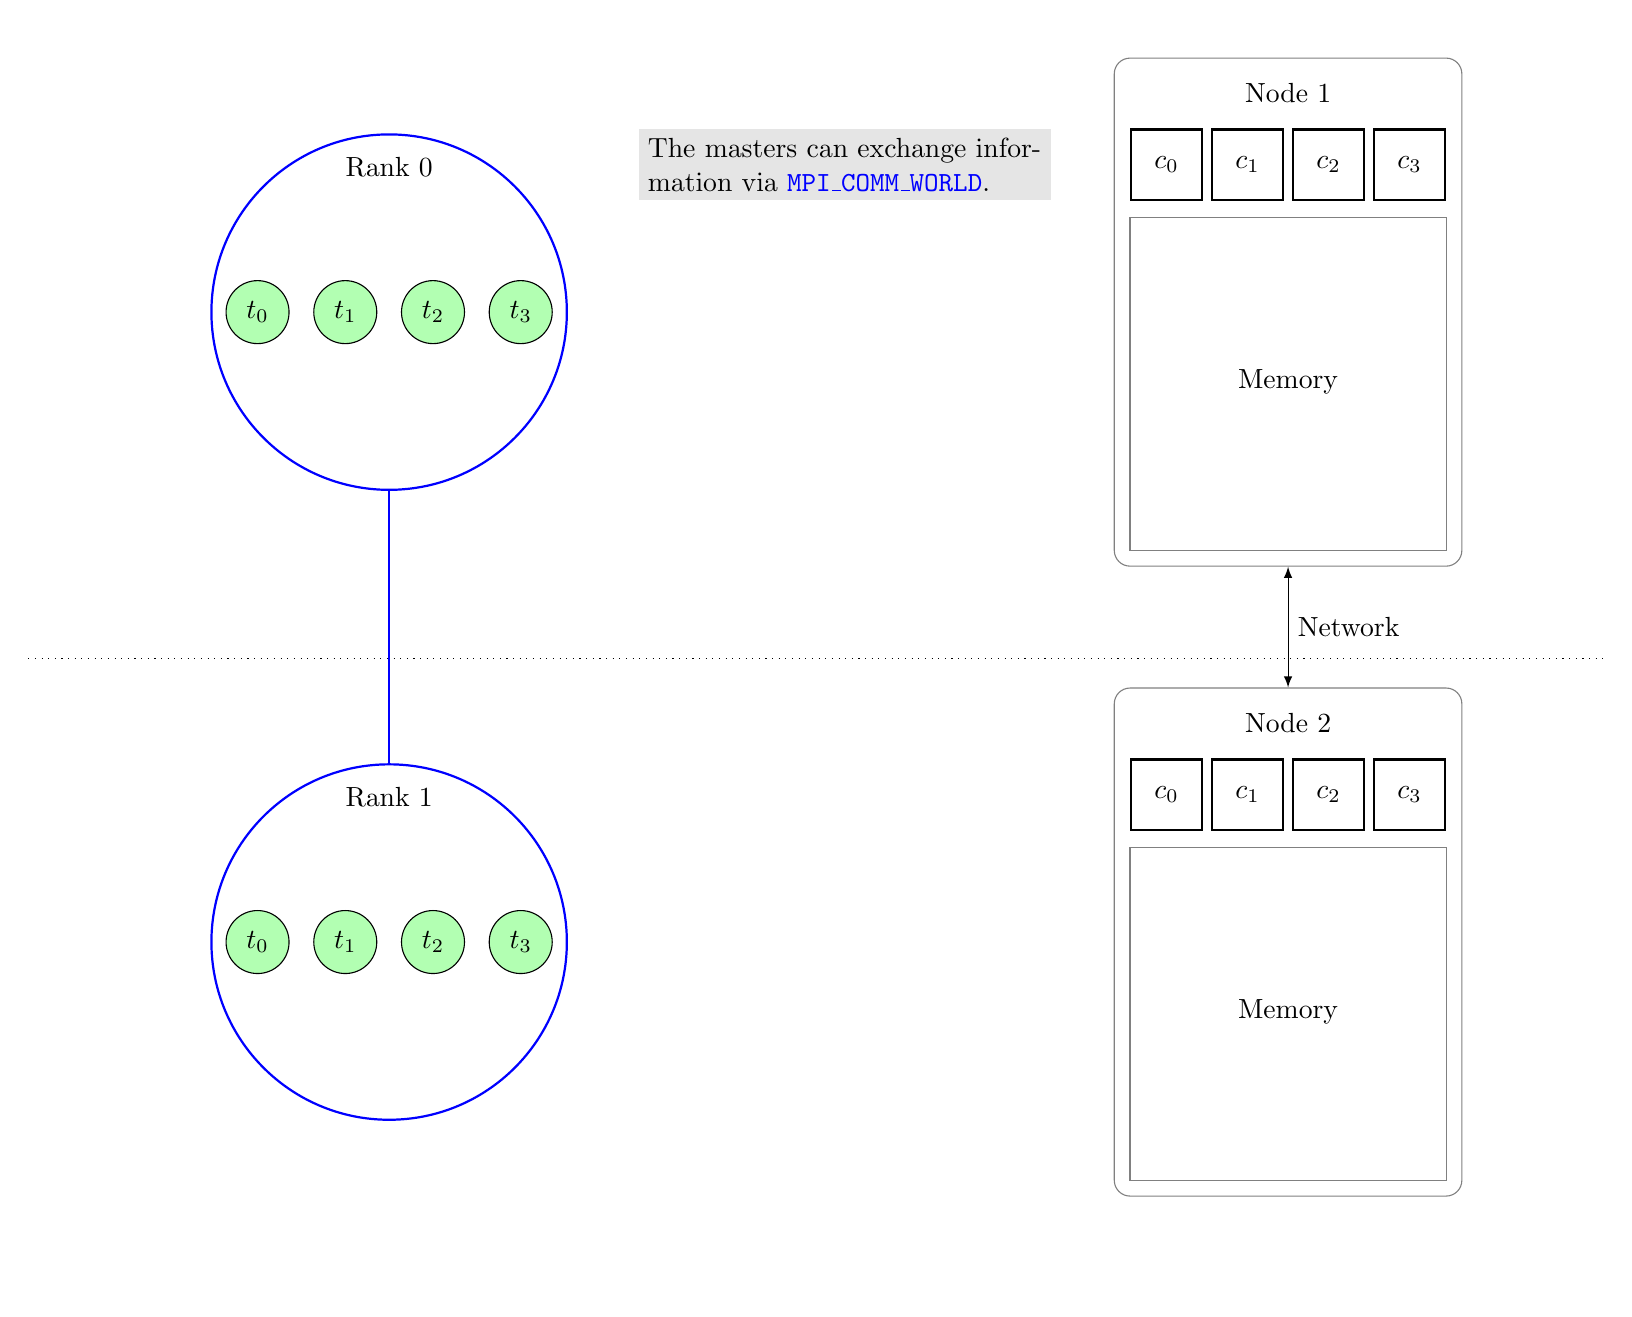
\begin{tikzpicture}[
		>=latex,
	]

	\pic {base={global}};

	% Master process with 4 threads
	\pic[left=7cm of n1] {master={1/running}};
	\pic[left=7cm of n2] {master={2/running}};
	\draw[thick,blue] (n1-master) -- (n2-master);

	\node (text) [fill=gray!20,left=1cm of n1-c,text width=5cm]
		{The masters can exchange information via 
		\textcolor{blue}{\texttt{MPI\_COMM\_WORLD}}.};

	%\draw[->] (text.170) to[out=180-45,in=180] ($(n1-master)!0.5!(n2-master)$);

\end{tikzpicture}
\end{adjustbox}
\end{figure}
\end{frame}

\begin{frame}[fragile]
\begin{figure}[h]
\begin{adjustbox}{max totalsize={\textwidth}{\textheight},center}
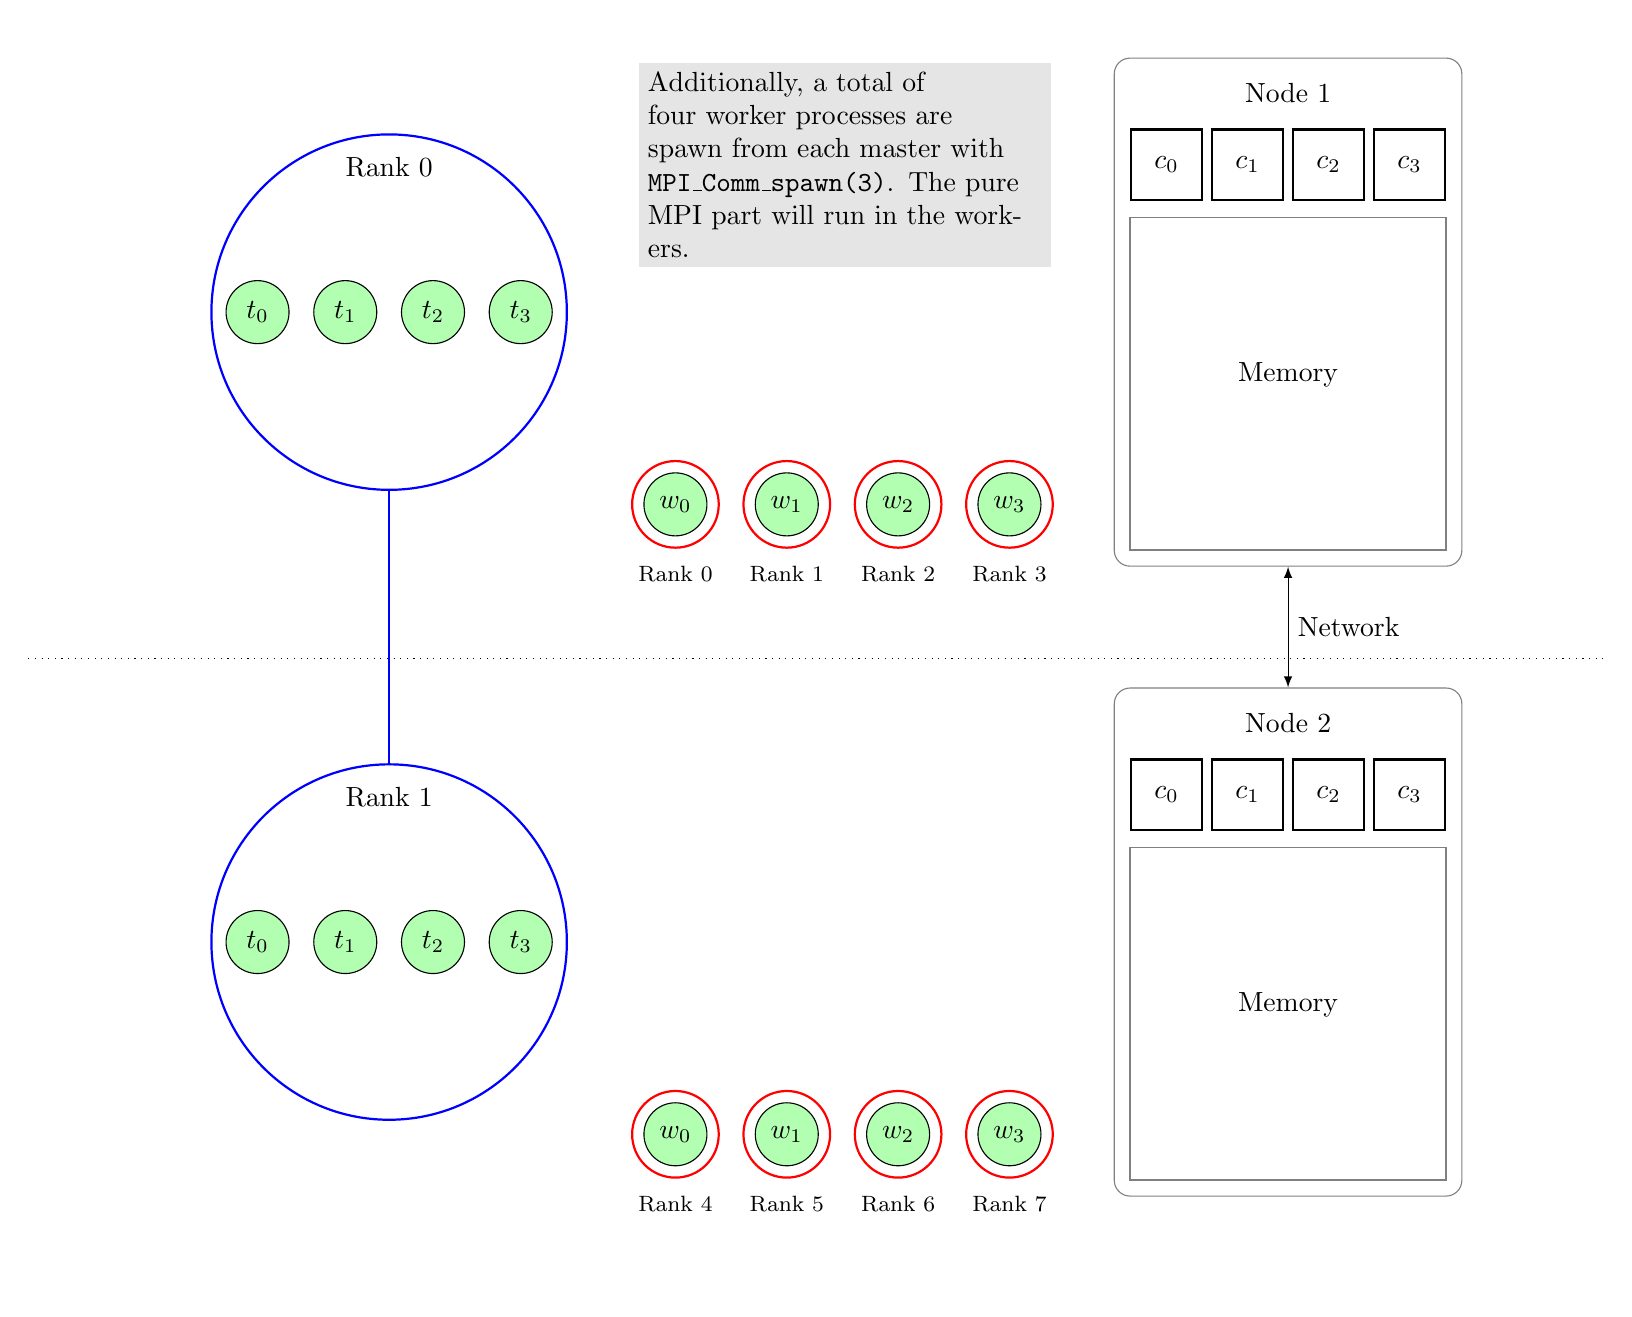
\begin{tikzpicture}[
		>=latex,
	]

	\pic {full={running/running}};

	\node[draw=gray,
				fill=white,
				inner sep=0mm,
				fit=(n1-mp)(n1-mn),
				] (n1-sm)	{Memory};

	\node[draw=gray,
				fill=white,
				inner sep=0mm,
				fit=(n2-mp)(n2-mn),
				] (n2-sm)	{Memory};

	\draw[thick,blue] (n1-master) -- (n2-master);

	\node (text) [fill=gray!20,left=1cm of n1-c,text width=5cm]
		{Additionally, a total of four worker processes are spawn from each master 
		with \texttt{MPI\_Comm\_spawn(3)}. The pure MPI part will run in the 
		workers.};


\end{tikzpicture}
\end{adjustbox}
\end{figure}
\end{frame}

\begin{frame}[fragile]
\begin{figure}[h]
\begin{adjustbox}{max totalsize={\textwidth}{\textheight},center}
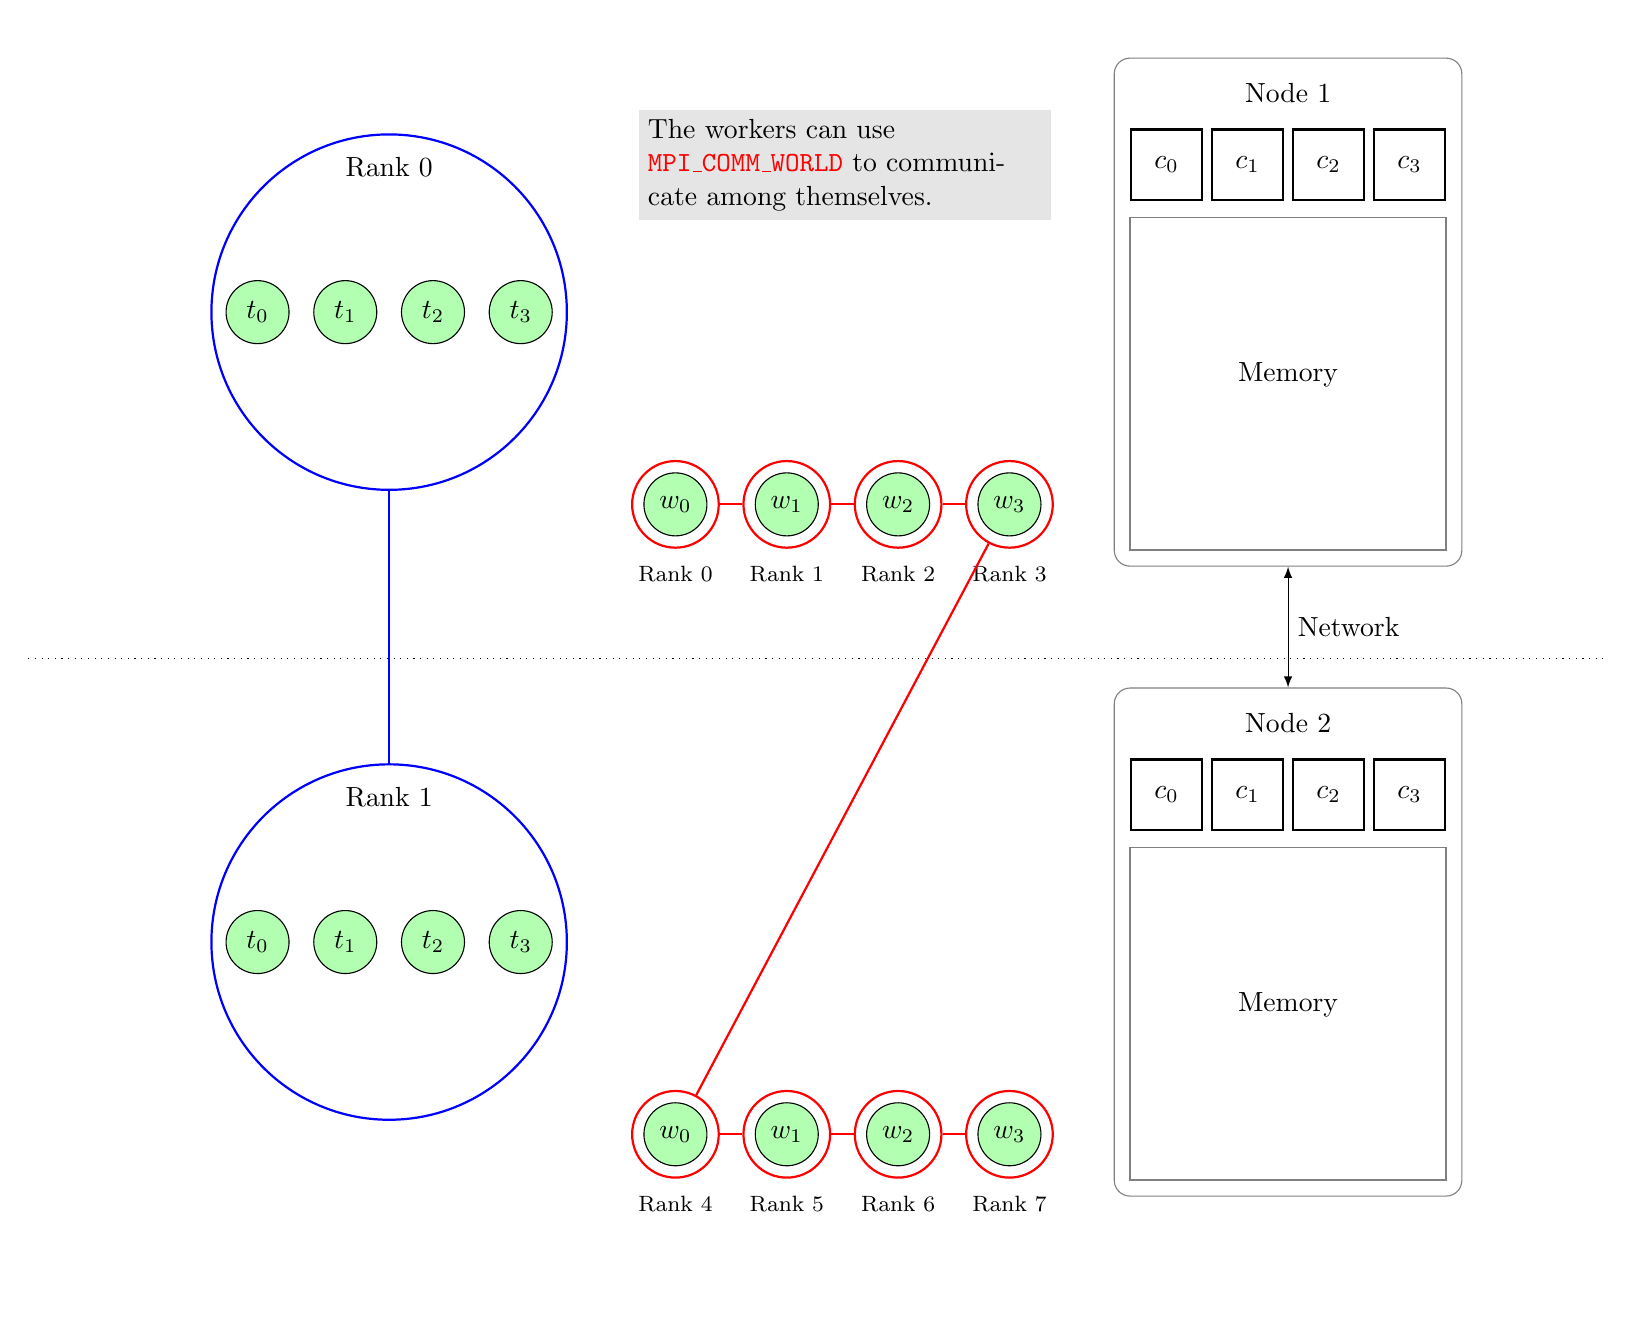
\begin{tikzpicture}[
		>=latex,
	]

	%\pic {base={global}};
	\pic {full={running/running}};

	\node[draw=gray,
				fill=white,
				inner sep=0mm,
				fit=(n1-mp)(n1-mn),
				] (n1-sm)	{Memory};

	\node[draw=gray,
				fill=white,
				inner sep=0mm,
				fit=(n2-mp)(n2-mn),
				] (n2-sm)	{Memory};

	\draw[thick,blue] (n1-master) -- (n2-master);
	\draw[red,thick] (n1-w0) -- (n1-w1) -- (n1-w2) -- (n1-w3);
	\draw[red,thick] (n2-w0) -- (n2-w1) -- (n2-w2) -- (n2-w3);
	\draw[red,thick] (n1-w3) -- (n2-w0);

	\node (text) [fill=gray!20,left=1cm of n1-c,text width=5cm]
		{The workers can use \textcolor{red}{\texttt{MPI\_COMM\_WORLD}} to 
		communicate among themselves.};

\end{tikzpicture}
\end{adjustbox}
\end{figure}
\end{frame}

\begin{frame}[fragile]
\begin{figure}[h]
\begin{adjustbox}{max totalsize={\textwidth}{\textheight},center}
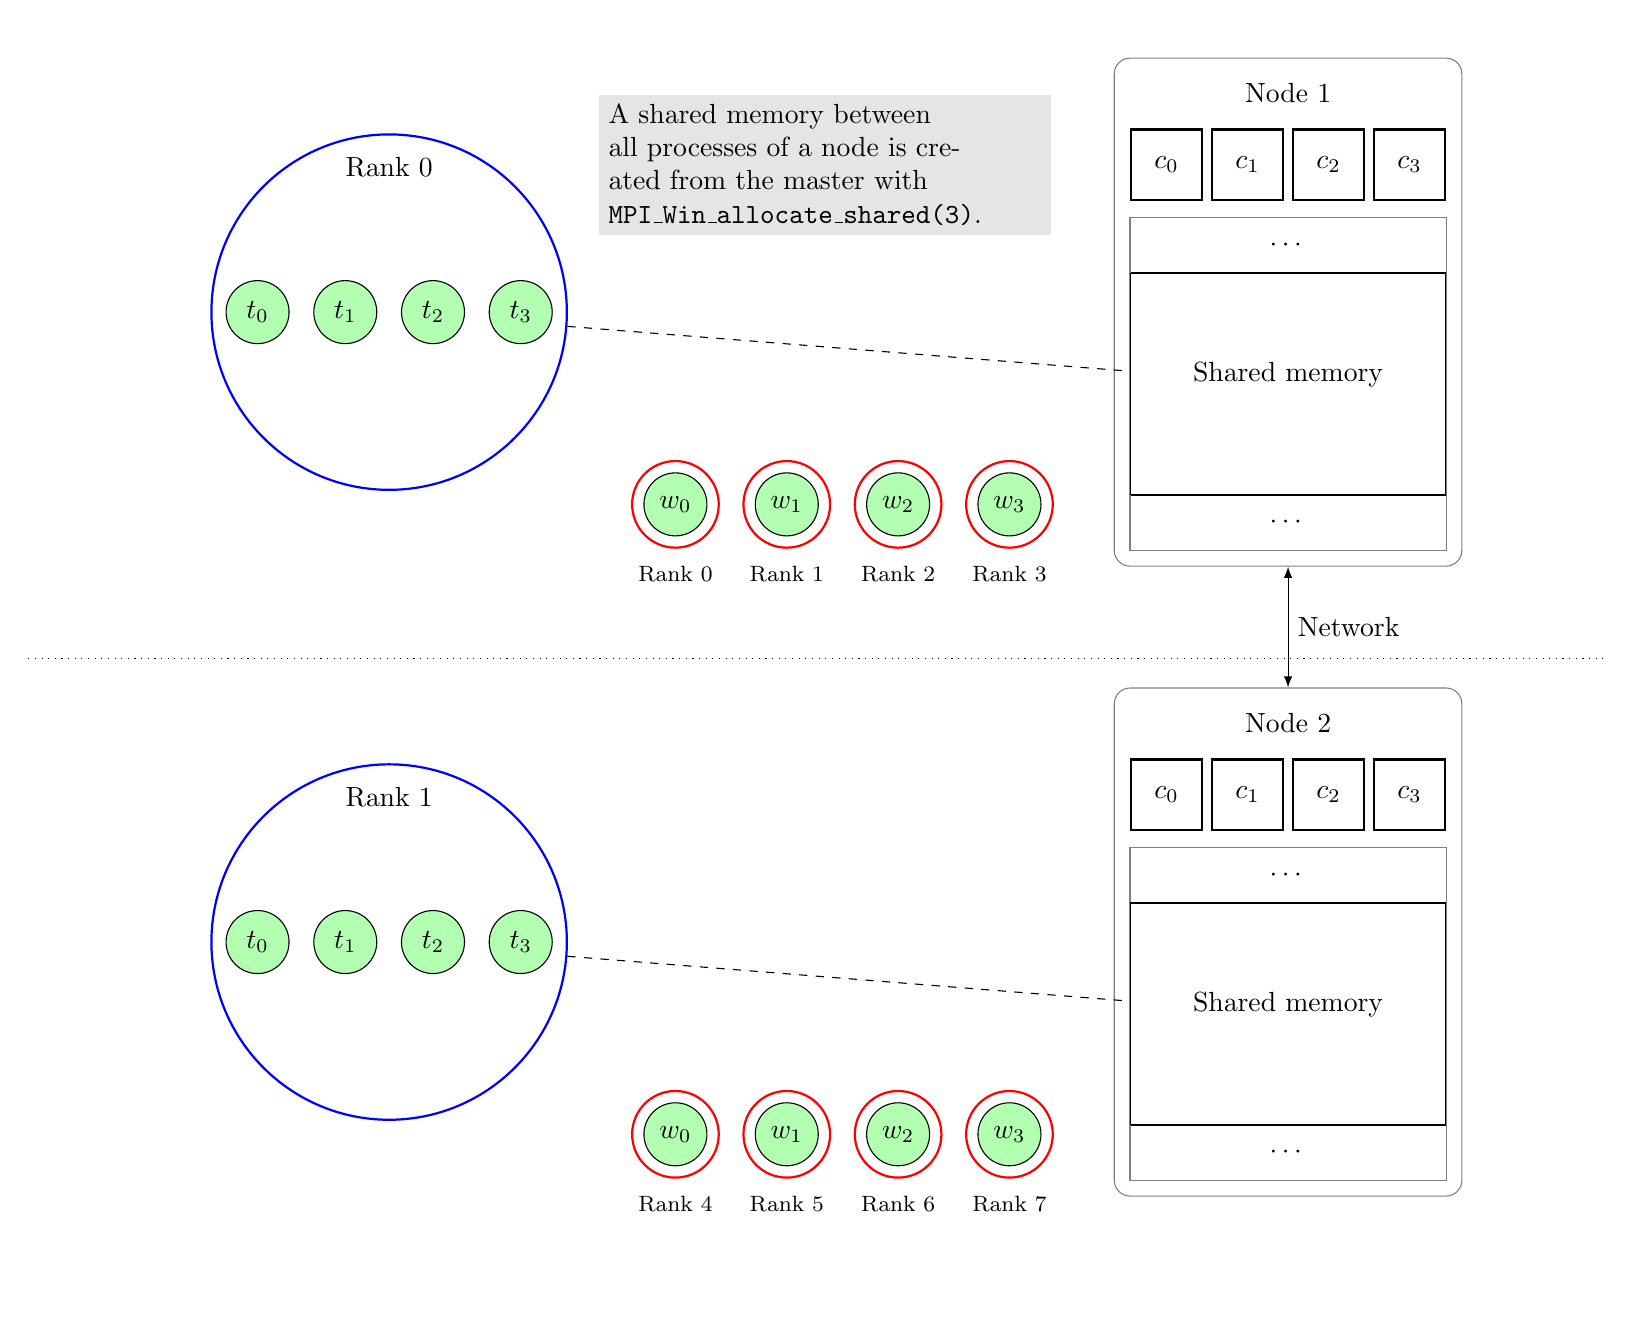
\begin{tikzpicture}[
		>=latex,
	]

	\pic {full={running/running}};

	\node[draw,
				fill=white,
				inner sep=0mm,
				fit=(n1-m0)(n1-m3),
				] (n1-sm)	{Shared memory};

	\node[draw,
				fill=white,
				inner sep=0mm,
				fit=(n2-m0)(n2-m3),
				] (n2-sm)	{Shared memory};

	% Draw lines from master to mem
	\draw[dashed] (n1-master) -- (n1-sm);
	\draw[dashed] (n2-master) -- (n2-sm);

	\node (text) [fill=gray!20,left=1cm of n1-c,text width=5.5cm]
		{A shared memory between all processes of a node is created from the master 
		with \texttt{MPI\_Win\_allocate\_shared(3)}.};


\end{tikzpicture}
\end{adjustbox}
\end{figure}
\end{frame}

\begin{frame}[fragile]
\begin{figure}[h]
\begin{adjustbox}{max totalsize={\textwidth}{\textheight},center}
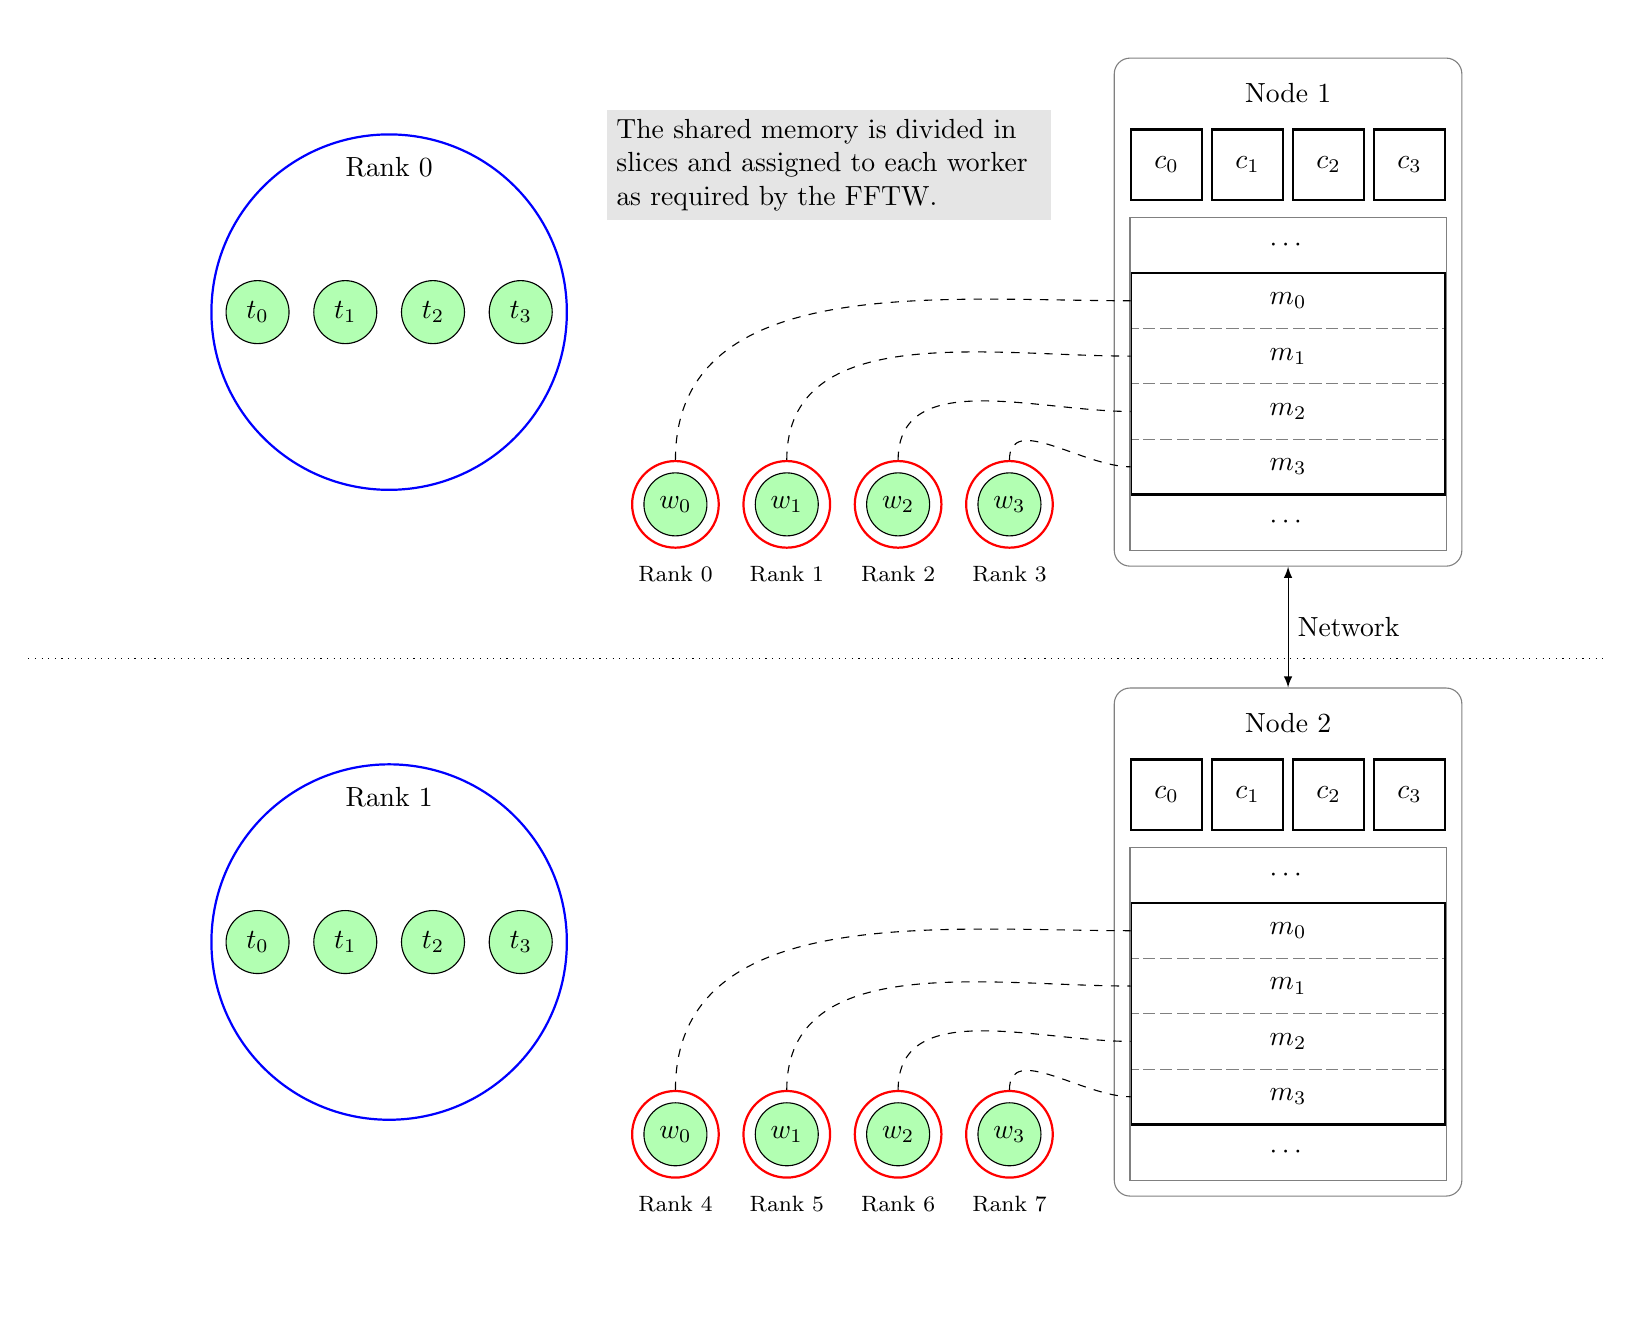
\begin{tikzpicture}[
		>=latex,
	]

	\pic {full={running/running}};

	\node (text) [fill=gray!20,left=1cm of n1-c,text width=5.4cm]
		{The shared memory is divided in slices and assigned to each worker as 
		required by the FFTW.};

	% Draw shared memory lines
	\foreach \n in {1,2}
		\foreach \i in {0,...,3}
			\draw[dashed] (n\n-w\i) to[out=90,in=180] (n\n-m\i);


\end{tikzpicture}
\end{adjustbox}
\end{figure}
\end{frame}

\begin{frame}[fragile]
\begin{figure}[h]
\begin{adjustbox}{max totalsize={\textwidth}{\textheight},center}
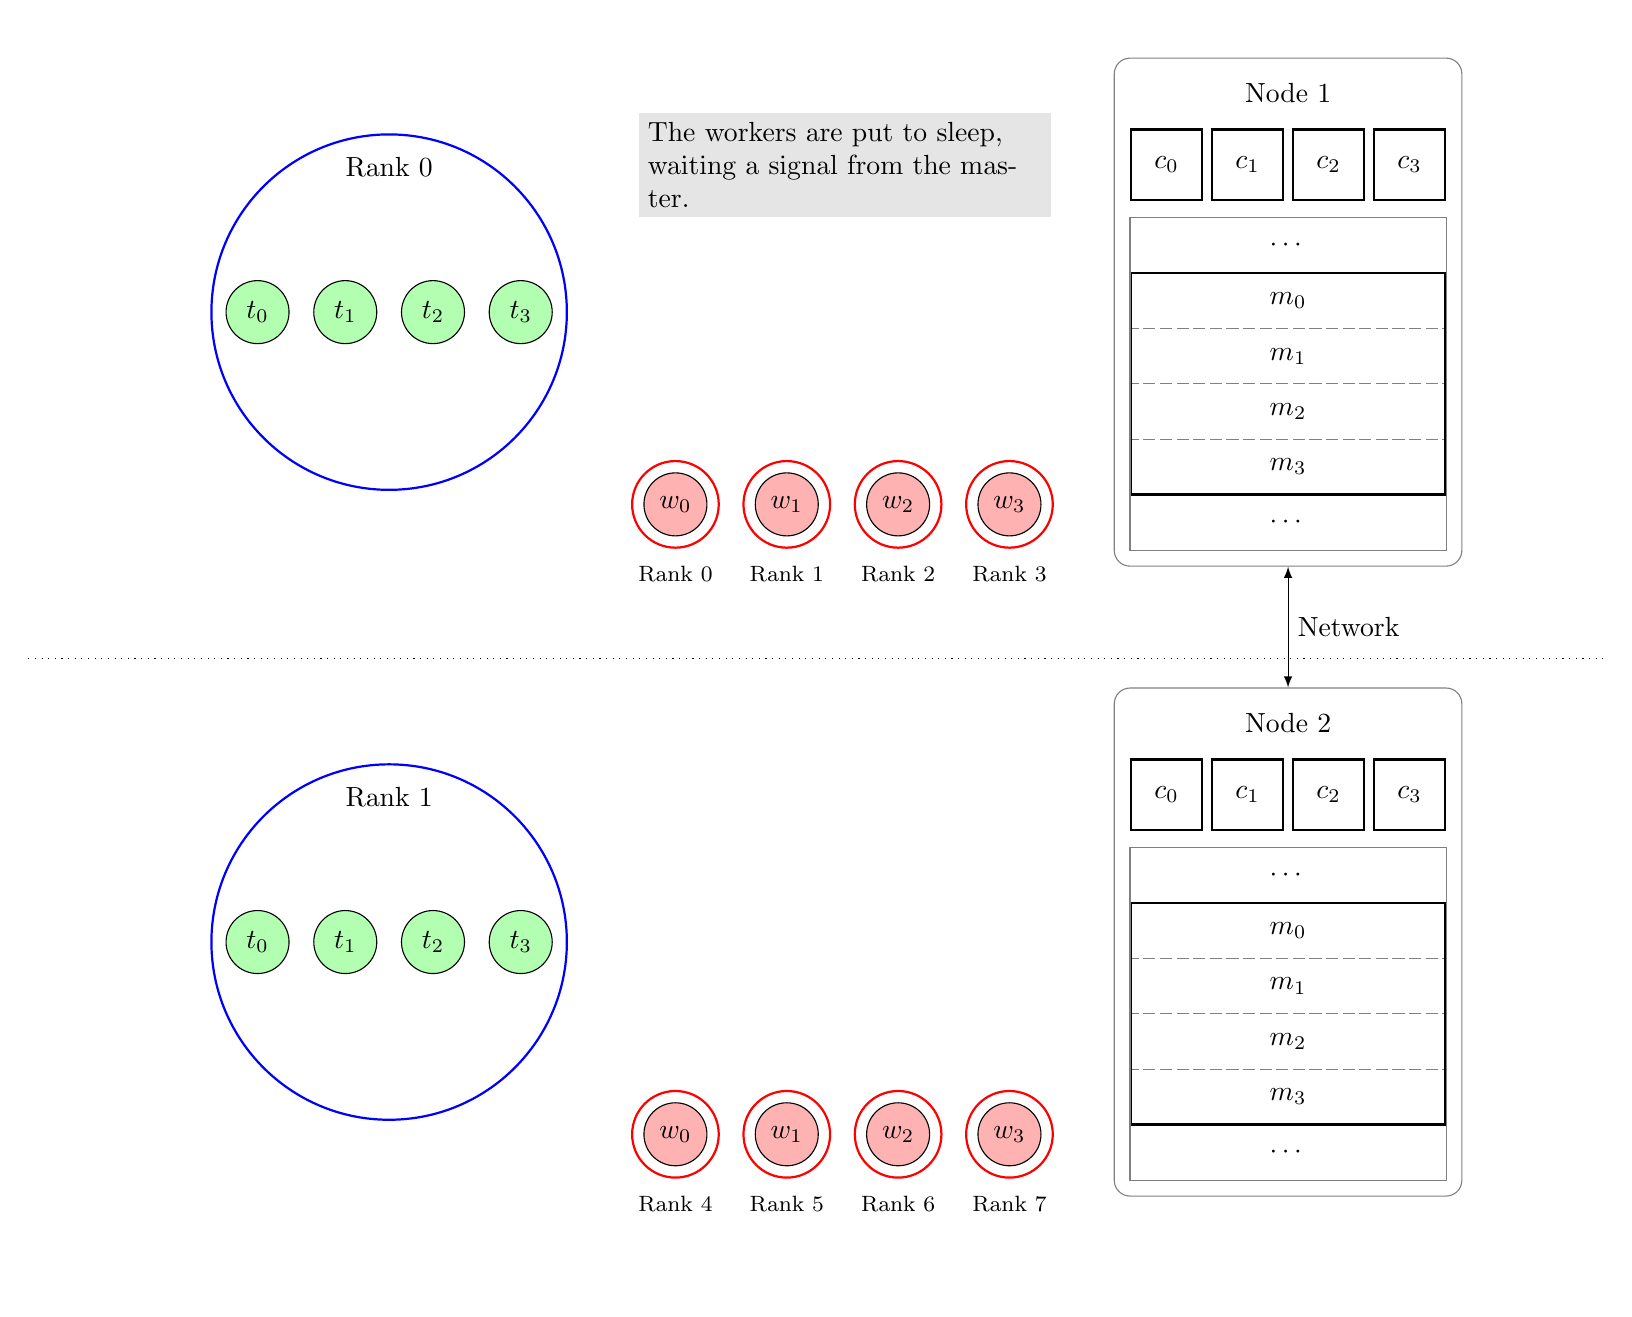
\begin{tikzpicture}[
		>=latex,
	]

	\pic {full={running/stopped}};

	\node (text) [fill=gray!20,left=1cm of n1-c,text width=5cm]
		{The workers are put to sleep, waiting a signal from the master.};

\end{tikzpicture}
\end{adjustbox}
\end{figure}
\end{frame}

\begin{frame}[fragile]
\begin{figure}[h]
\begin{adjustbox}{max totalsize={\textwidth}{\textheight},center}
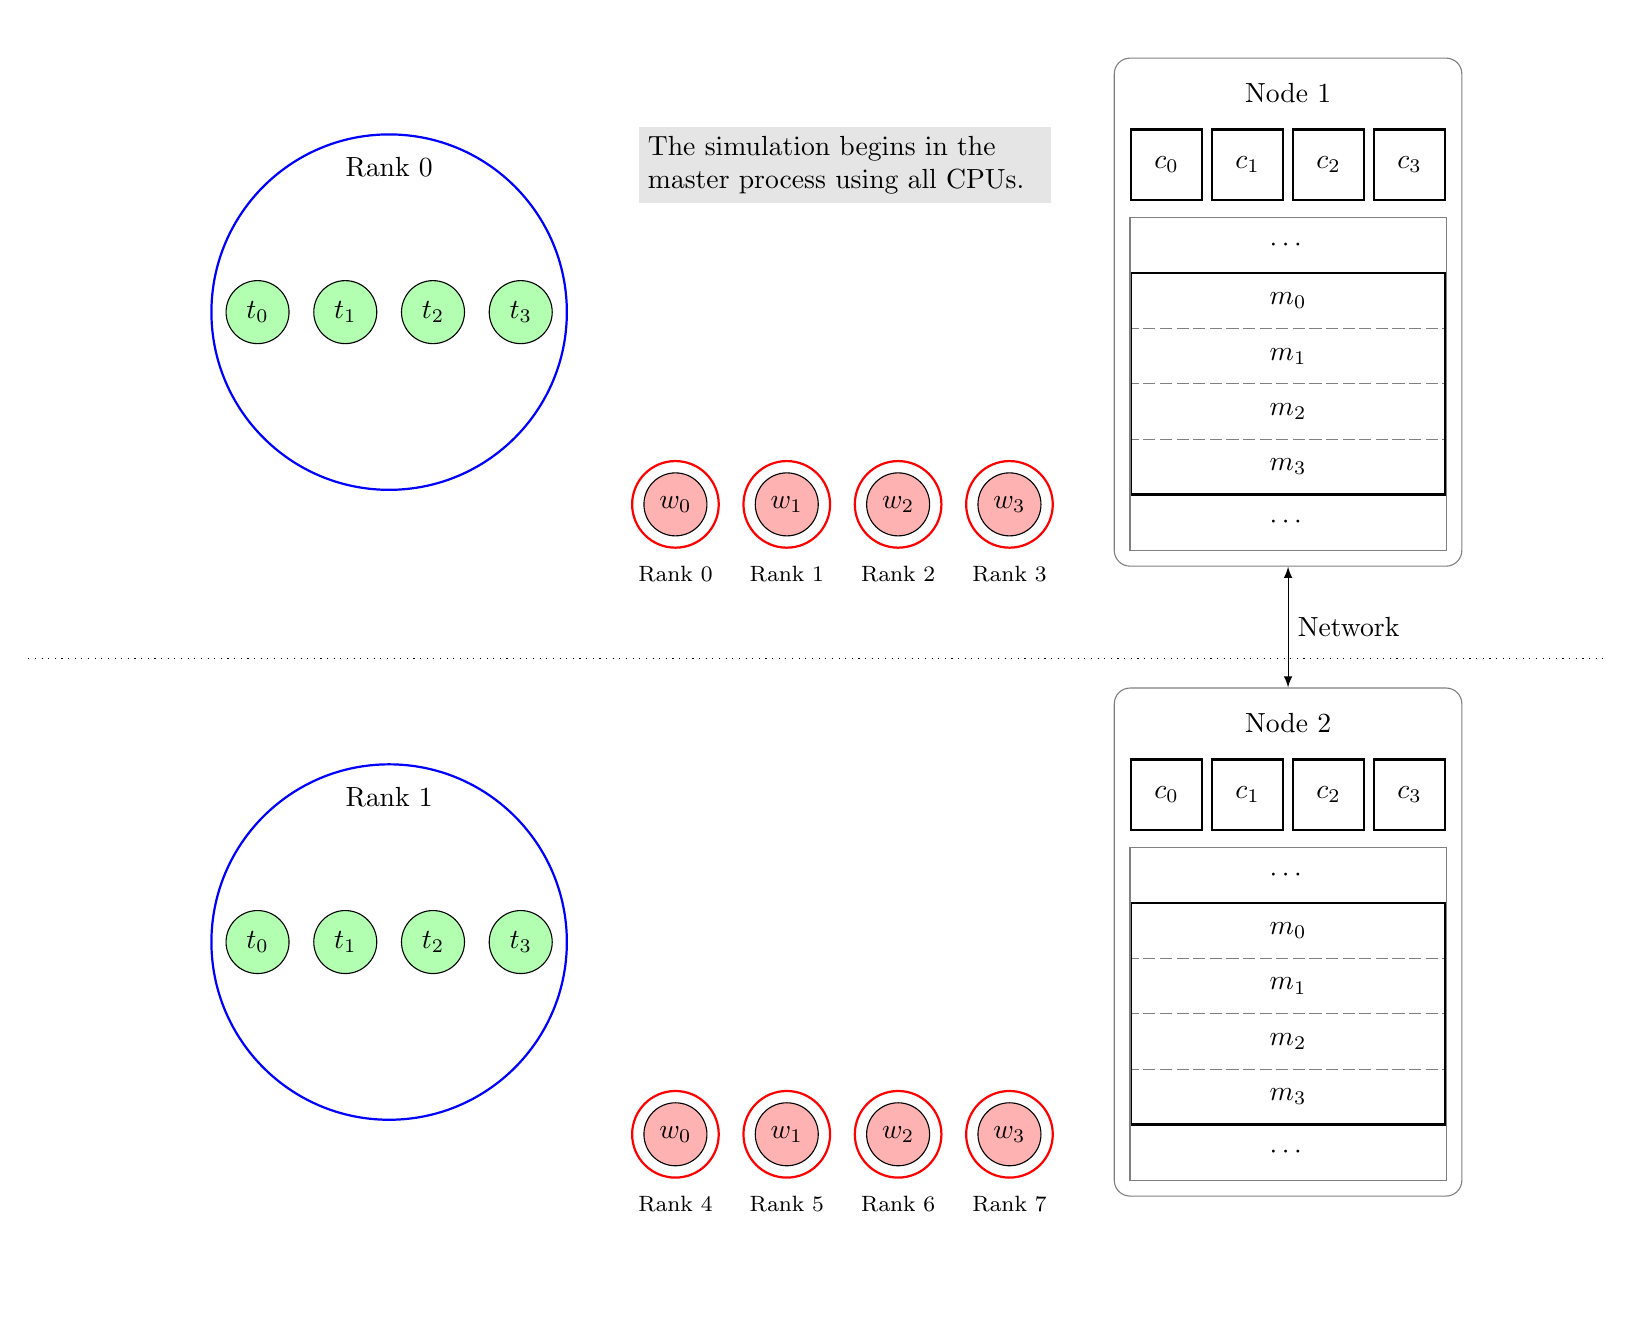
\begin{tikzpicture}[
		>=latex,
	]


	\pic {full={running/stopped}};

	\node (text) [fill=gray!20,left=1cm of n1-c,text width=5cm]
		{The simulation begins in the master process using all CPUs.};

	%\foreach \n in {1,2}
	%	\foreach \c in {0,1,2,3}
	%		\draw (n\n-t\c) -- (n\n-c\c);

\end{tikzpicture}
\end{adjustbox}
\end{figure}
\end{frame}

\begin{frame}[fragile]
\begin{figure}[h]
\begin{adjustbox}{max totalsize={\textwidth}{\textheight},center}
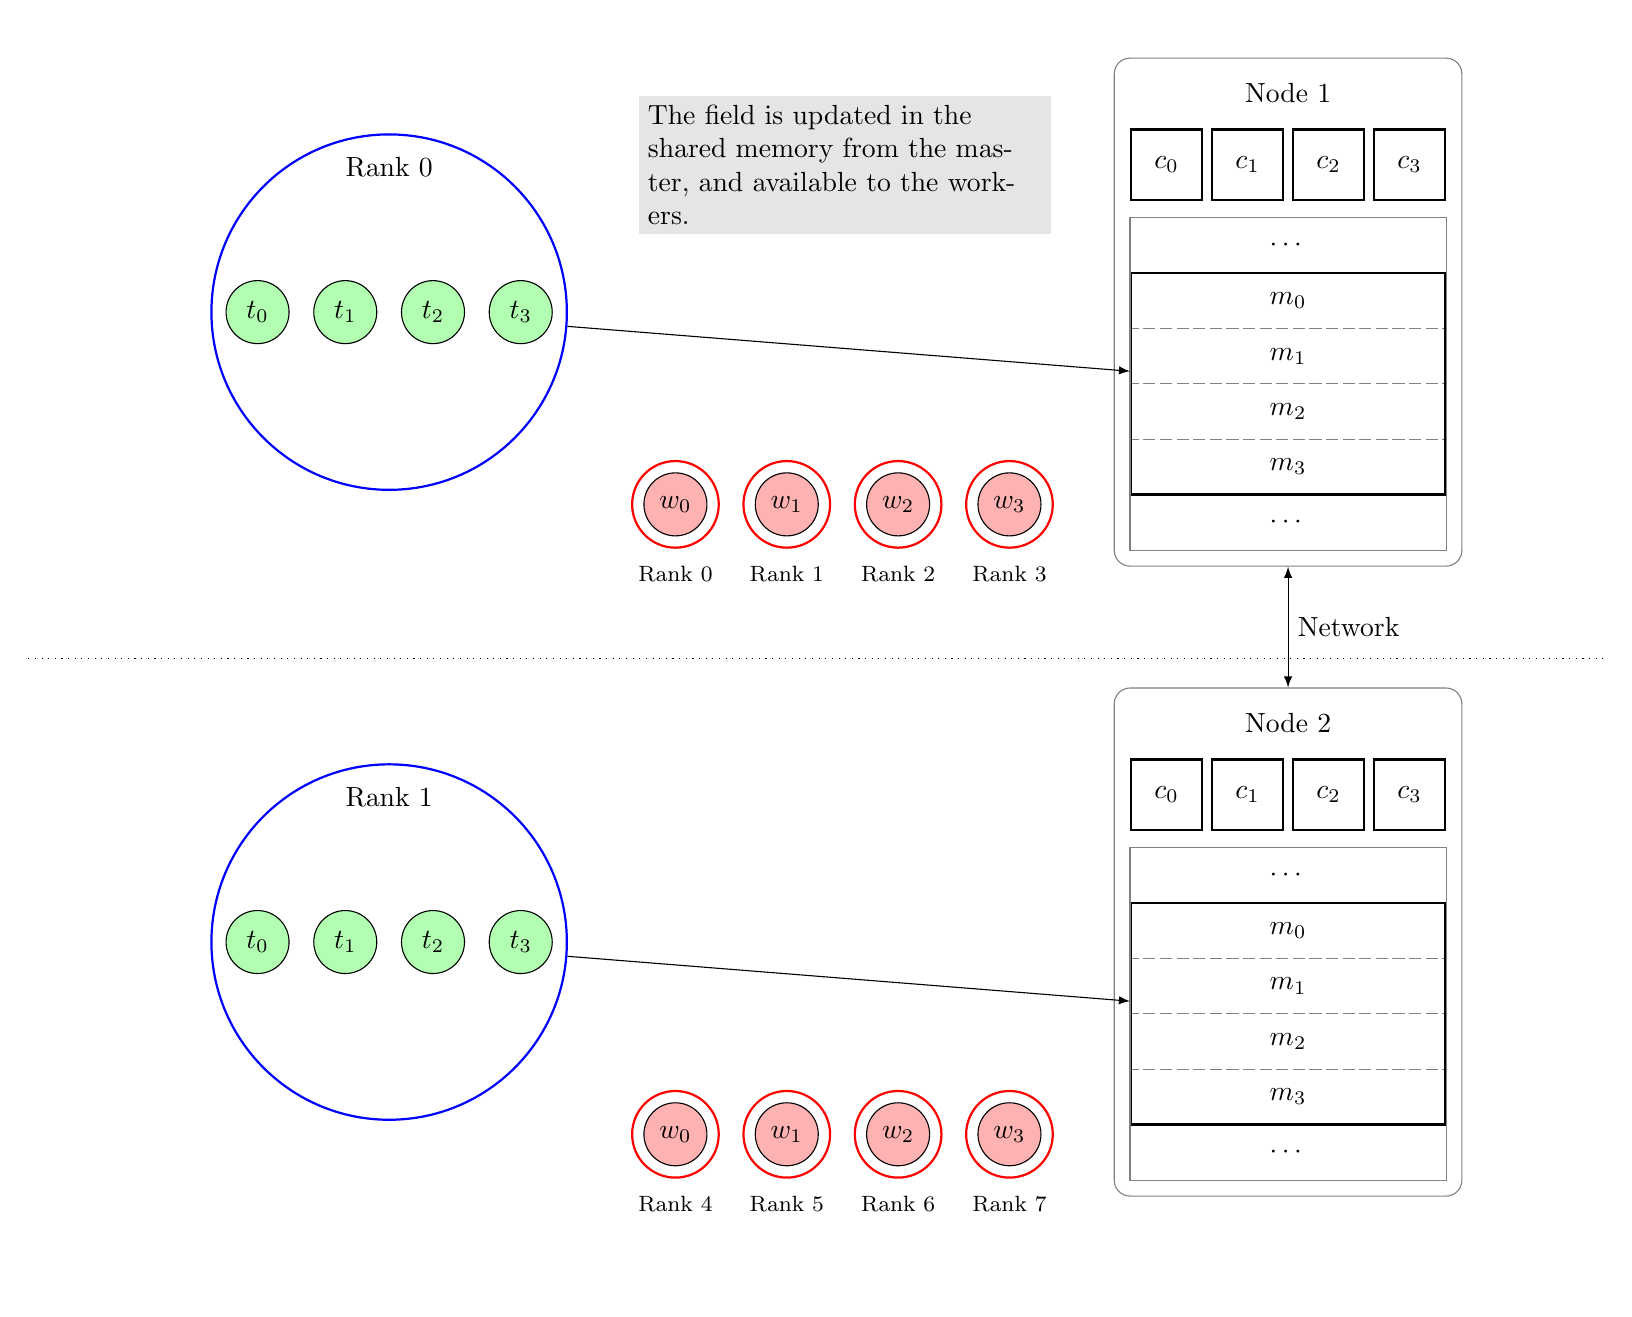
\begin{tikzpicture}[
		>=latex,
	]

	\pic {full={running/stopped}};

	\foreach \n in {1,2}
		\draw[->] (n\n-master) -- (n\n-m);

	\node (text) [fill=gray!20,left=1cm of n1-c,text width=5cm]
		{The field is updated in the shared memory from the master, and available to 
		the workers.};

\end{tikzpicture}
\end{adjustbox}
\end{figure}
\end{frame}

\begin{frame}[fragile]
\begin{figure}[h]
\begin{adjustbox}{max totalsize={\textwidth}{\textheight},center}
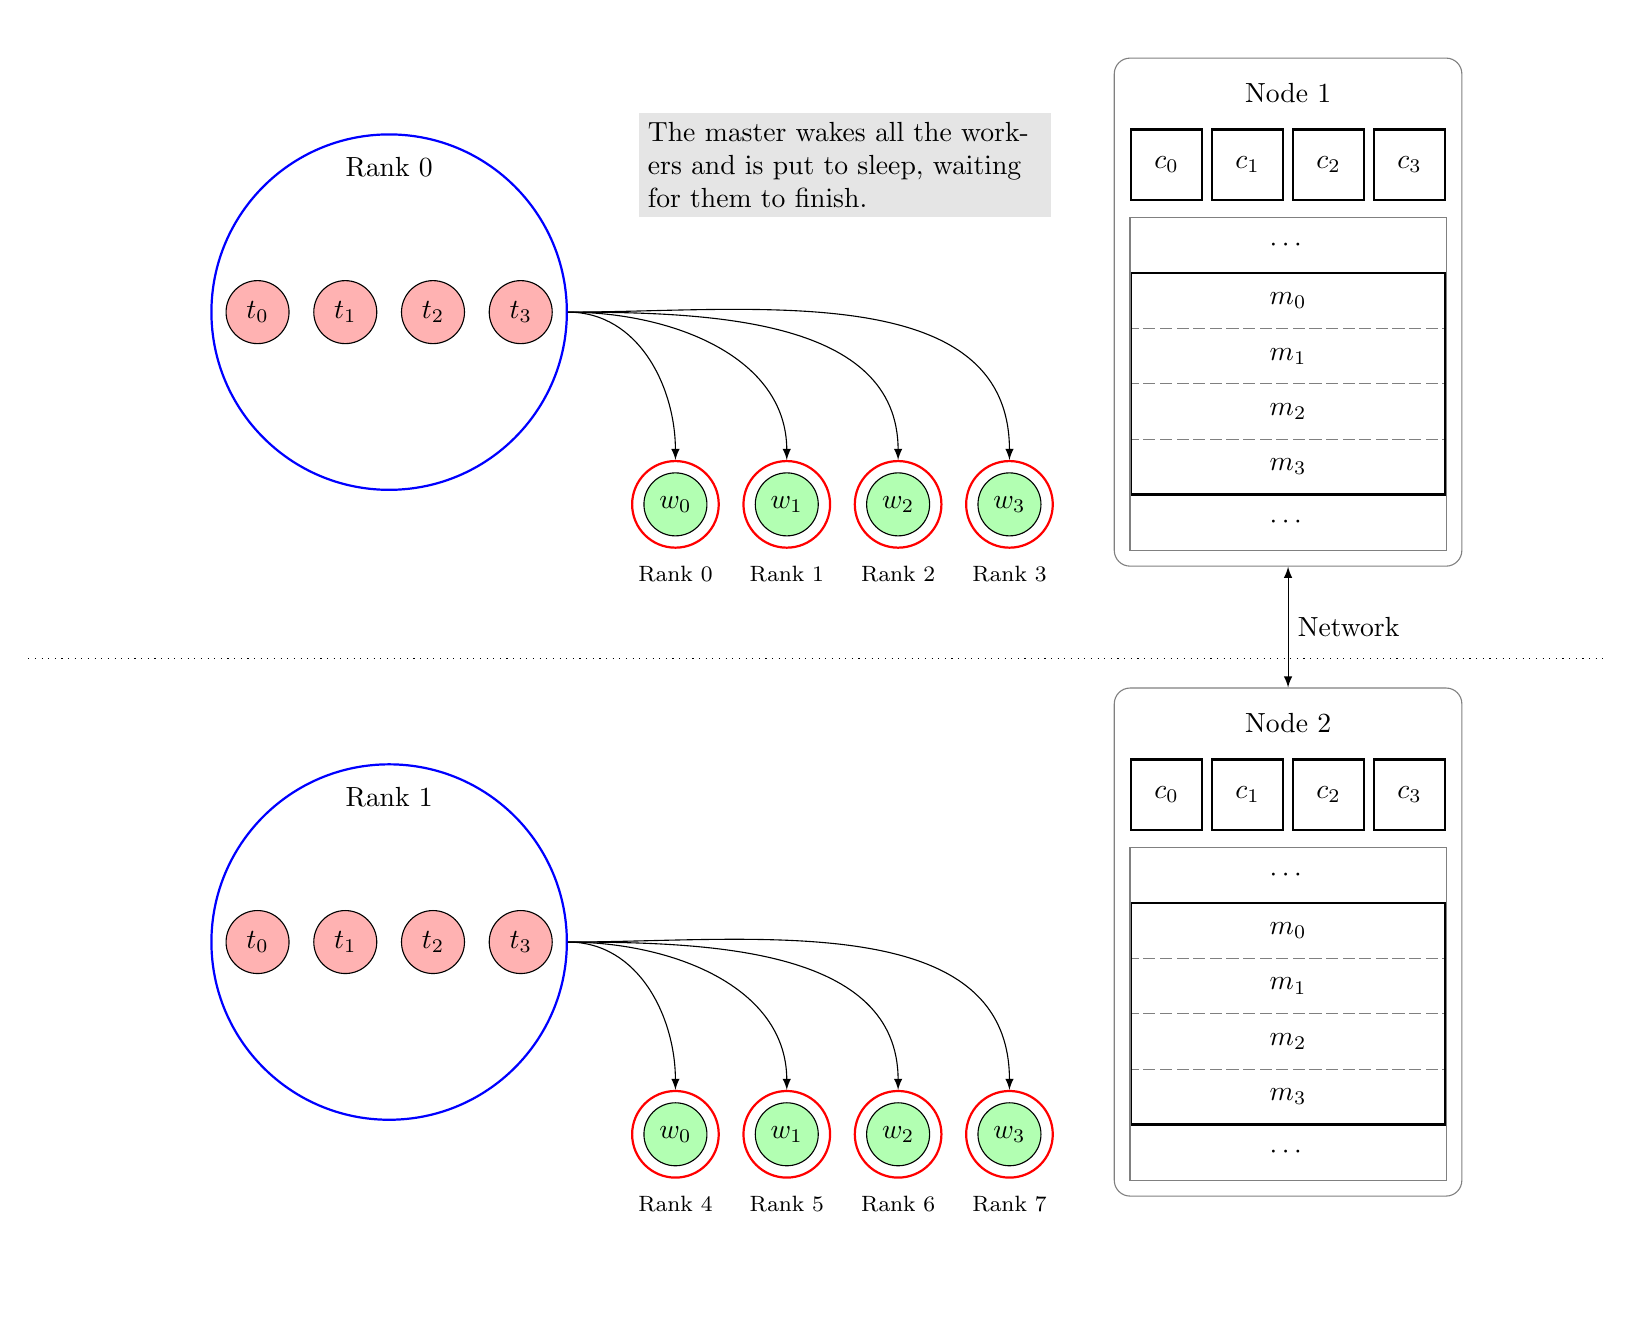
\begin{tikzpicture}[
		>=latex,
	]

	\pic {full={stopped/running}};

	% Draw lines from master to the workers
	\foreach \n in {1,2}
		\foreach \i in {0,...,3}
			\draw[->] (n\n-master) to[out=0,in=90] (n\n-w\i);

	\node (text) [fill=gray!20,left=1cm of n1-c,text width=5cm]
		{The master wakes all the workers and is put to sleep, waiting for them to 
		finish.};

\end{tikzpicture}
\end{adjustbox}
\end{figure}
\end{frame}

\begin{frame}[fragile]
\begin{figure}[h]
\begin{adjustbox}{max totalsize={\textwidth}{\textheight},center}
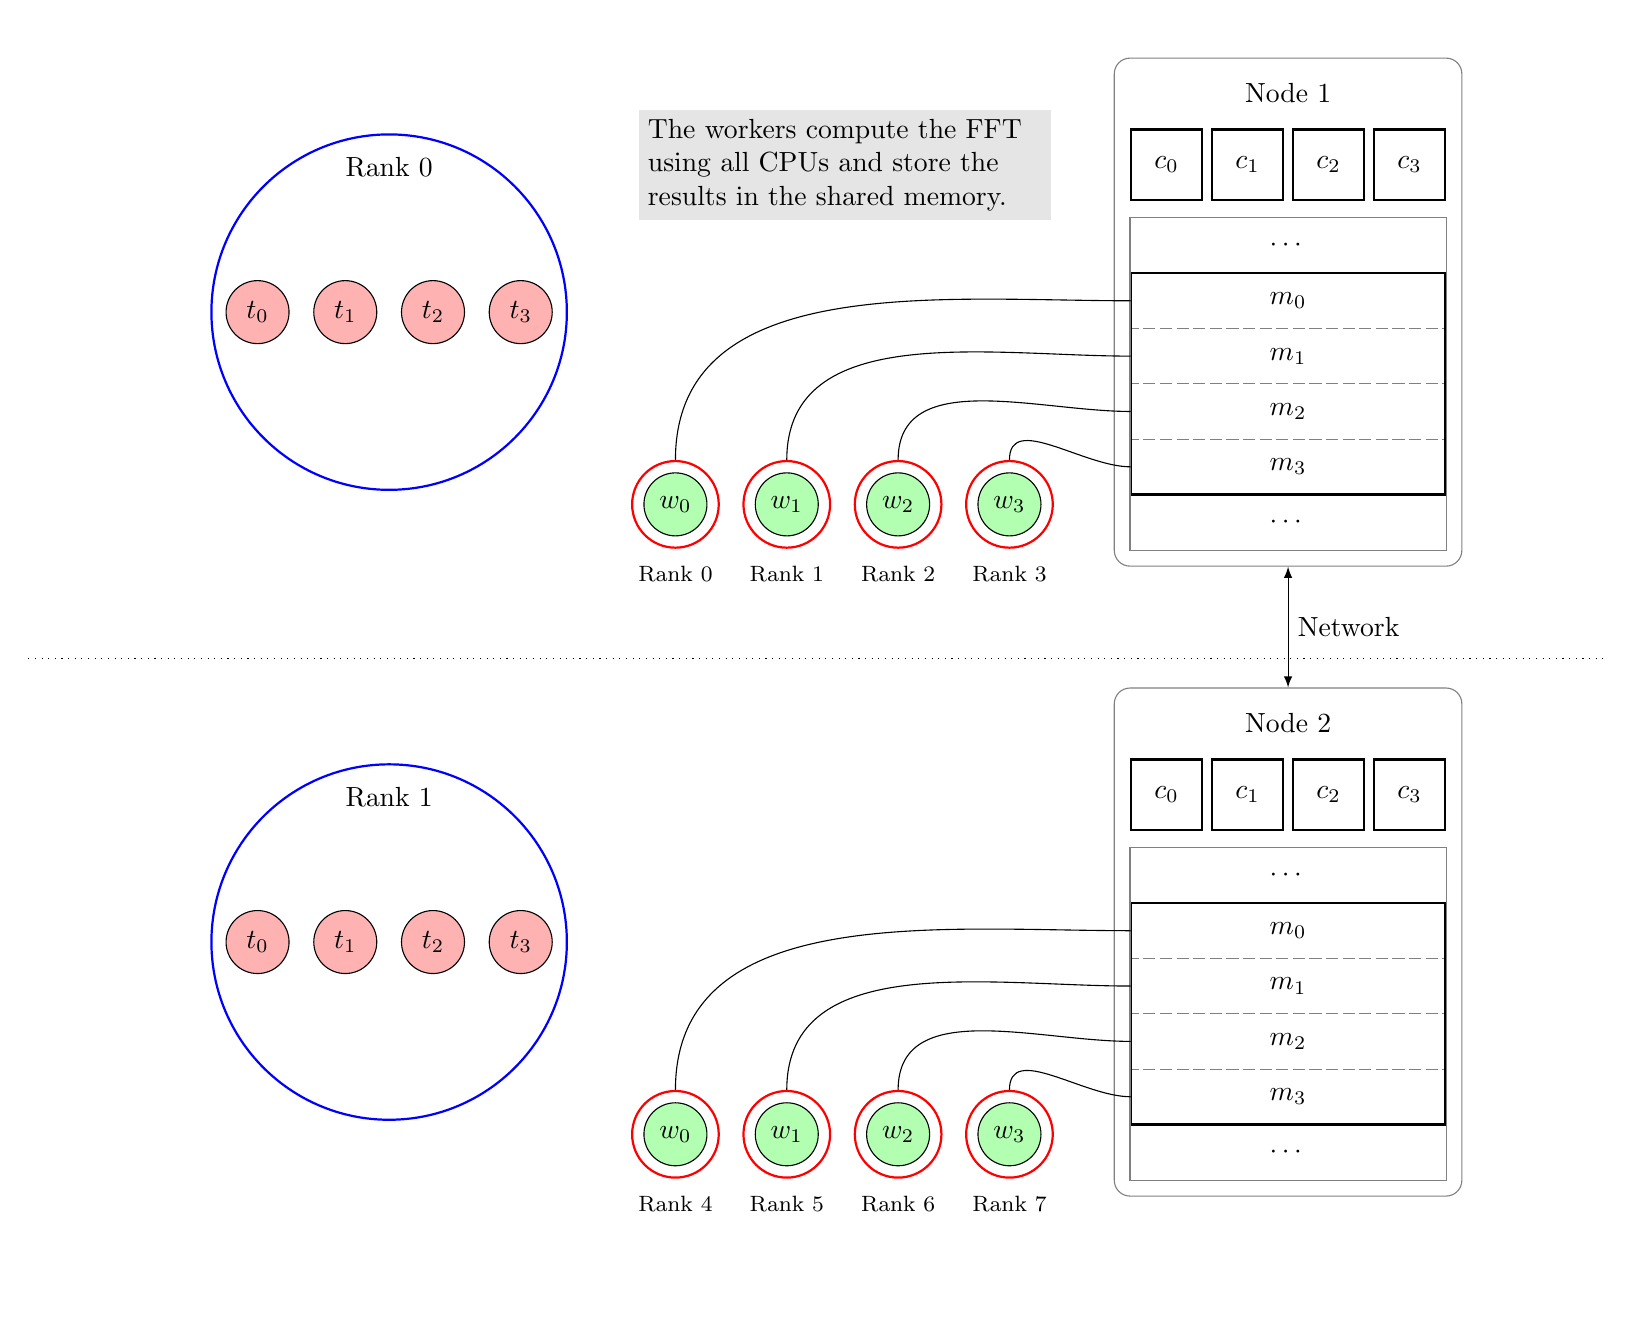
\begin{tikzpicture}[
		>=latex,
	]

	\pic {full={stopped/running}};

	\foreach \n in {1,2}
	{
		% Draw lines from the workers to mem
		\foreach \i in {0,...,3}
			\draw (n\n-w\i) to[out=90,in=180] (n\n-m\i.west);
	}

	\node (text) [fill=gray!20,left=1cm of n1-c,text width=5cm]
		{The workers compute the FFT using all CPUs and store the results in the 
		shared memory.};

\end{tikzpicture}
\end{adjustbox}
\end{figure}
\end{frame}

\begin{frame}[fragile]
\begin{figure}[h]
\begin{adjustbox}{max totalsize={\textwidth}{\textheight},center}
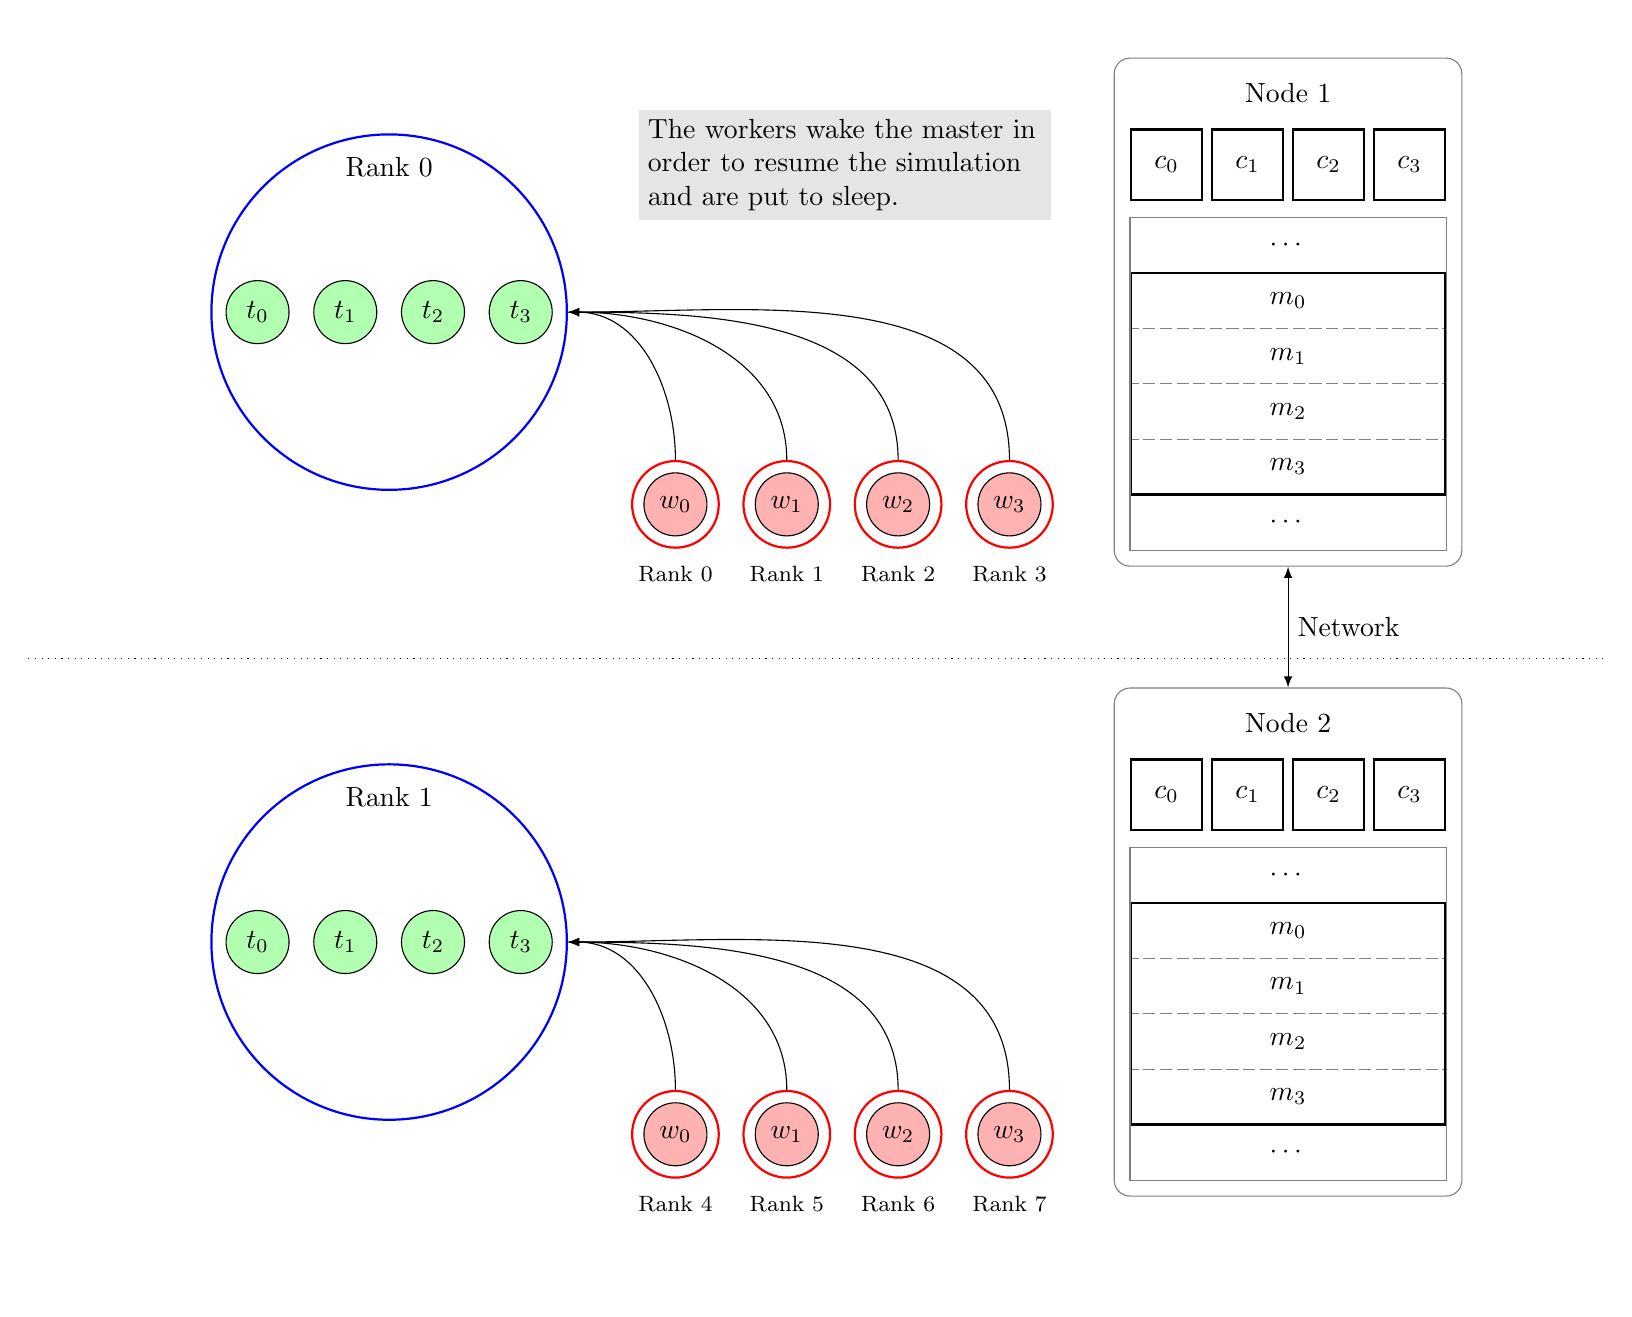
\begin{tikzpicture}[
		>=latex,
	]

	\pic {full={running/stopped}};

	% Draw lines from the workers to mem
	\foreach \n in {1,2}
	{
		\foreach \i in {0,...,3}
			\draw[->] (n\n-w\i) to[out=90,in=0] (n\n-master);
	}

	\node (text) [fill=gray!20,left=1cm of n1-c,text width=5cm]
		{The workers wake the master in order to resume the simulation and are put 
		to sleep.};

\end{tikzpicture}
\end{adjustbox}
\end{figure}
\end{frame}

\begin{frame}[fragile]
\begin{figure}[h]
\begin{adjustbox}{max totalsize={\textwidth}{\textheight},center}
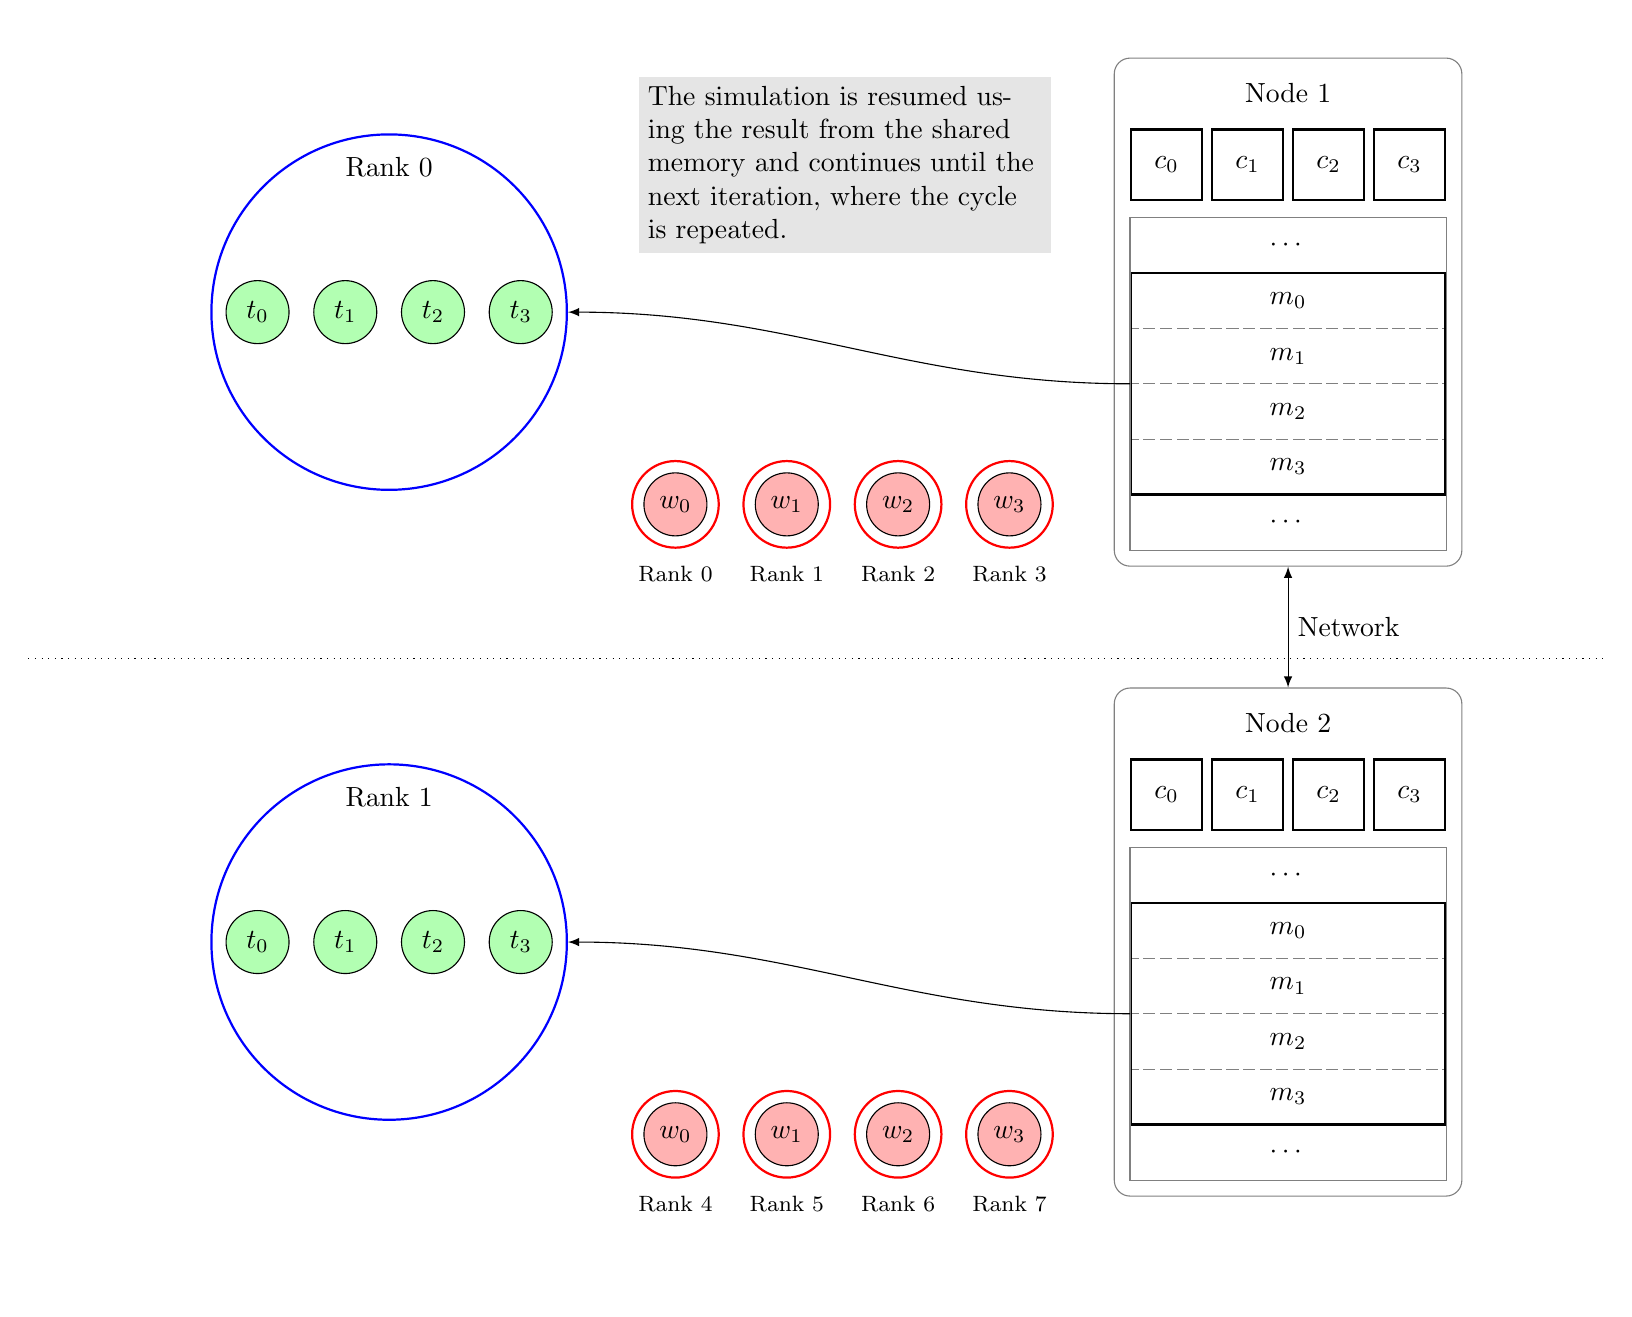
\begin{tikzpicture}[
		>=latex,
	]

	\pic {full={running/stopped}};

	\foreach \n in {1,2}
		\draw[<-] (n\n-master) to[out=0,in=180] (n\n-m);

	\node (text) [fill=gray!20,left=1cm of n1-c,text width=5cm]
		{The simulation is resumed using the result from the shared memory and 
		continues until the next iteration, where the cycle is repeated.};

\end{tikzpicture}
\end{adjustbox}
\end{figure}
\end{frame}


\begin{frame}{Comments}

Notice that at all times there are always as many active threads or processes as 
CPUs available---we have no oversubscription (except at the initialization).

\vspace{1em}

The current mechanism to stop and resume the processes is implemented using the 
signals SIGSTOP and SIGCONT.

\end{frame}



\begin{frame}{Results: Time per iteration}
\begin{figure}[ht]%{{{
\centering
\begin{adjustbox}{max totalsize={.9\textwidth}{.7\textheight},center}
\begin{tikzpicture}
	\begin{axis}[
		xmode=log,
		ymode=log,
		log basis x=2,
		log basis y=2,
		%xticklabels={0,1,2,4,8,16,32},
		xticklabel style={
			/pgf/number format/fixed,
			/pgf/number format/precision=5
		},
		scaled x ticks=false,
		log ticks with fixed point,
		grid=major,
		xmin=0,
		ymin=0,
		xlabel=Number of nodes,
		ylabel=Time per iteration (s),
		height=8cm,
		width=1\textwidth,
		legend pos=outer north east,
		/tikz/font=\small]
		\addplot+ table [
			x = P,
			y = mean,
			col sep=tab,
		] {perf/notap/csv/time.csv};
		\addplot+ table [
			x = P,
			y = mean,
			col sep=tab] {perf/tap/csv/time.csv};
		\legend{TAP disabled,TAP enabled}
	\end{axis}
\end{tikzpicture}
\end{adjustbox}
\caption{Time per iteration with 32K$\times$32K gridpoints, 2M particles.  Each 
node has 48 CPUs, using 48 CPUs/node for the main simulation, 32 CPUs/node for 
the solver.}
\label{fig:time}
\end{figure}%}}}
\end{frame}

\begin{frame}{Results: Strong scaling}
\begin{figure}[ht]%{{{
\centering
\begin{adjustbox}{max totalsize={.9\textwidth}{.7\textheight},center}
\begin{tikzpicture}
	\begin{axis}[
		xmode=log,
		ymode=log,
		log basis x=2,
		log basis y=2,
		log ticks with fixed point,
		xticklabels={0,1,2,4,8,16,32},
		grid=major,
		xmin=0,
		ymin=0,
		xlabel=Number of nodes,
		ylabel=Speedup,
		height=8cm,
		width=0.7\textwidth,
		/tikz/font=\small]
		\addplot+ table [
			x = P,
			y = speedup,
			col sep=tab] {perf/notap/csv/time.csv};
		\addplot+ table [
			x = P,
			y = speedup,
			col sep=tab] {perf/tap/csv/time.csv};
	\end{axis}
\end{tikzpicture}
\begin{tikzpicture}
	\begin{axis}[
		xmode=log,
		log basis x=2,
		xticklabels={0,1,2,4,8,16,32},
		grid=major,
		xmin=0,
		ymin=0,
		xlabel=Number of nodes,
		ylabel=Efficiency,
		height=8cm,
		width=0.7\textwidth,
		legend pos=outer north east,
		/tikz/font=\small]
		\addplot+ table [
			x = P,
			y = efficiency,
			col sep=tab] {perf/notap/csv/time.csv};
		\addplot+ table [
			x = P,
			y = efficiency,
			col sep=tab] {perf/tap/csv/time.csv};
		\legend{TAP disabled,TAP enabled}
	\end{axis}
\end{tikzpicture}
\end{adjustbox}
\caption{Strong scaling with 32K$\times$32K gridpoints, 2M particles.  Each node 
has 48 CPUs, using 48 CPUs/node for the main simulation, 32 CPUs/node for the 
solver.}
\label{fig:strong-scaling}
\end{figure}%}}}
\end{frame}


\begin{frame}{Trace comparison}
\begin{figure}
\centering
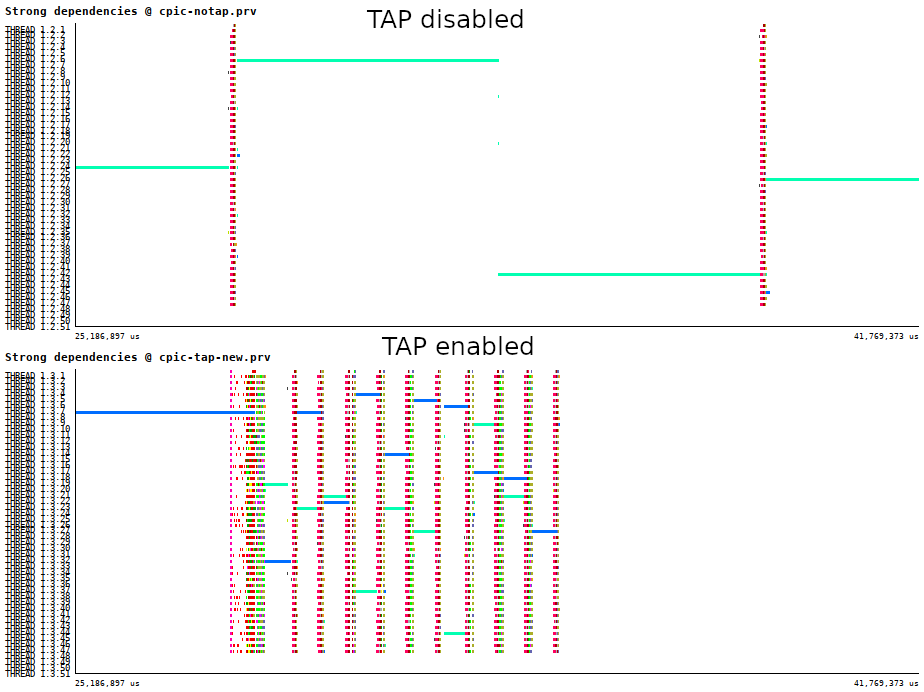
\includegraphics[width=.95\textwidth]{tap/trace-comp}
\end{figure}
Notice the traces have the same time scale in the X axis.
\end{frame}

\begin{frame}{Requirements for using TAP}

To determine if you could benefit from using TAP, divide your application in two 
parts: The hybrid parallelization uses all CPUs in all nodes, and scales 
properly. And the pure part, which uses only MPI parallelization and thus only 
one CPU is used per process.  Then, ensure that:
\vspace{1em}

\begin{itemize}
\item The pure MPI part is the bottleneck.
\item There would be an increase in performance if more MPI processes run the 
pure part.
\item A shared region can be used to communicate the hybrid and pure parts.
\item You don't want or can't introduce hybrid parallelization in the pure part.
\end{itemize}

\end{frame}

\end{document}
